\Chapter{ETUDE DU SAUT D'UNE ROUE CYR}\label{sec:Theme1}
\begin{table}[htbp]
  \centering
  \caption{Constantes et variables de la modélisation du saut d'une roue Cyr}
  \begin{tabular}{|c|l|}
    \hline \rowcolor[gray]{0.8}\color{black}
    Symbole         & Description\\
    $A$           & Aire de la section\\
   
    $E$           & Module d'Young du matériau\\
    $E_{p,g}$          & Energie potentielle gravitationnelle\\
    $E_{tot}$          & Energie mécanique totale\\
    $F$             & Force de compression appliquée à la roue\\
    $g$     & Accélération gravitationnelle\\
    $H_{max}$          & Hauteur de saut maximale\\
    $I$           & Moment quadratique de la section\\
    $k$             & raideur équivalente de la roue\\
    $m_r$          & Masse de la roue\\
    
    $R$       & Rayon médian de la roue\\
    $r_1$ & Rayon interne de section pour une section circulaire\\
    $r_2$             & rayon externe de section pour une section circulaire\\
    $\rho$           & Masse volumique du matériau\\ \hline
  \end{tabular}
  \label{tab:Definitions}
\end{table}


\section{Etude théorique}
\subsection{Description du mouvement}
La roue Cyr est comprimée par une force verticale $F$ exercée selon l'axe de son diamètre puis relâchée. Une partie de l'énergie de déformation élastique est transformée en saut. On notera $H_{max}$ la hauteur correspondant à l'énergie potentielle par laquelle s'élève le centre de gravité de la roue depuis sa position au repos à sa hauteur maximale.


\subsubsection{Hypothèses}
\begin{itemize}
    \item On considère que le support contre lequel la roue est comprimée est parfaitement rigide.
    \item On néglige la force de traînée de l'air.
    \item La répartition des masses est idéalisée
\end{itemize}

\subsubsection{Modèle deux degrés de liberté}
On modélise la roue Cyr par deux masses ponctuelles égales $m_r/2$ reliées par un ressort de rigidité $k$ et de longueur à vide $2R$, où $R$ correspond au rayon médian de la roue. \\
La rigidité équivalente de la roue est donnée par \cite{yangkim}:
\begin{equation}
    k=\frac{4\pi EI}{(\pi^2 -8)R^3},
    \label{eq:0}
\end{equation}

où $E$ est le module d'Young et $I$ est le moment moment quadratique de la section de la roue.

\\
 Les positions des masses sont reperées par les ordonnées $y_1(t)$ et $y_2(t)$.

\begin{figure}[htb]
\centering

%% Creator: Inkscape inkscape 0.92.2, www.inkscape.org
%% PDF/EPS/PS + LaTeX output extension by Johan Engelen, 2010
%% Accompanies image file 'repos2.eps' (pdf, eps, ps)
%%
%% To include the image in your LaTeX document, write
%%   \input{<filename>.pdf_tex}
%%  instead of
%%   \includegraphics{<filename>.pdf}
%% To scale the image, write
%%   \def\svgwidth{<desired width>}
%%   \input{<filename>.pdf_tex}
%%  instead of
%%   \includegraphics[width=<desired width>]{<filename>.pdf}
%%
%% Images with a different path to the parent latex file can
%% be accessed with the `import' package (which may need to be
%% installed) using
%%   \usepackage{import}
%% in the preamble, and then including the image with
%%   \import{<path to file>}{<filename>.pdf_tex}
%% Alternatively, one can specify
%%   \graphicspath{{<path to file>/}}
%% 
%% For more information, please see info/svg-inkscape on CTAN:
%%   http://tug.ctan.org/tex-archive/info/svg-inkscape
%%
\begingroup%
  \makeatletter%
  \providecommand\color[2][]{%
    \errmessage{(Inkscape) Color is used for the text in Inkscape, but the package 'color.sty' is not loaded}%
    \renewcommand\color[2][]{}%
  }%
  \providecommand\transparent[1]{%
    \errmessage{(Inkscape) Transparency is used (non-zero) for the text in Inkscape, but the package 'transparent.sty' is not loaded}%
    \renewcommand\transparent[1]{}%
  }%
  \providecommand\rotatebox[2]{#2}%
  \ifx\svgwidth\undefined%
    \setlength{\unitlength}{337.82993867bp}%
    \ifx\svgscale\undefined%
      \relax%
    \else%
      \setlength{\unitlength}{\unitlength * \real{\svgscale}}%
    \fi%
  \else%
    \setlength{\unitlength}{\svgwidth}%
  \fi%
  \global\let\svgwidth\undefined%
  \global\let\svgscale\undefined%
  \makeatother%
  \begin{picture}(1,0.62816437)%
    \put(0,0){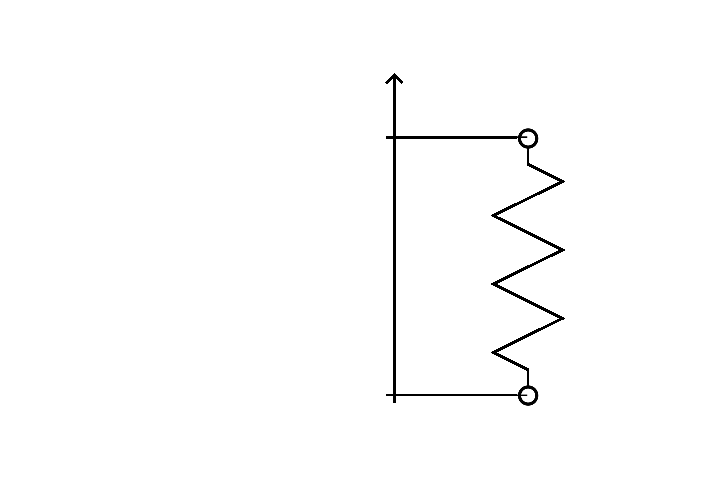
\includegraphics[width=\unitlength]{images_2ddl/repos2.eps}}%
    \put(0.53610169,0.57938811){\color[rgb]{0,0,0}\makebox(0,0)[lb]{\smash{$y$}}}%
    \put(0.29,0.46){\color[rgb]{0,0,0}\makebox(0,0)[lb]{\smash{$y_1=2R-\dfrac{m_r g}{2k}$}}}%
    \put(0.42,0.09){\color[rgb]{0,0,0}\makebox(0,0)[lb]{\smash{$y_2=0$}}}%
    \put(0.62490379,0.2696811){\color[rgb]{0,0,0}\makebox(0,0)[lb]{\smash{$k$}}}%
    \put(0.7581069,0.49168631){\color[rgb]{0,0,0}\makebox(0,0)[lb]{\smash{$\dfrac{m_r}{2}$}}}%
    \put(0.78030738,0.0698765){\color[rgb]{0,0,0}\makebox(0,0)[lb]{\smash{$\dfrac{m_r}{2}$}}}%
  \end{picture}%
\endgroup%

\caption{Système au repos. Le ressort de longueur à vide $2R$ et de raideur $k$ est écrasé par le poids de la masse supérieure.}
\label{fig:repos}
\end{figure}

\subsection{Limite en comportement linéaire}

A partir d'une certaine flèche $\delta$ imposée par une force de compression $F$, l'anneau ne se comporte plus de manière linéaire et la relation $F=k\delta$, où $k$ est la constante définie dans l'équation \ref{eq:0}, n'est plus valable. 
La valeur limite de $\delta$ au delà de laquelle on sort du domaine de comportement linéaire, est définie avec une étude éléments finis prenant en compte les non linéarités d'ordre géométrique, que l'on compare avec le modèle théorique linéaire (figure \ref{fig:lin1}). Dans cette étude, la roue est modélisée avec des éléments poutres, le déplacement $\delta$ est imposé comme paramètre d'entrée et la force $F$, relevée comme donnée de sortie, pour des raisons de convergence.

On considère qu'on sort de la zone de comportement linéaire lorsque la valeur absolue de l'erreur relative entre les deux modèles, $\epsilon=\frac{F_{éléments finis}-F_{théorique}}{F_{théorique}}$ dépasse 10\%. La limite du domaine de comportement linéaire correspond donc à $\frac{delta}{R}<0.1$

\begin{figure}[h]
\centering
%% Creator: Inkscape inkscape 0.92.2, www.inkscape.org
%% PDF/EPS/PS + LaTeX output extension by Johan Engelen, 2010
%% Accompanies image file 'lineaire.eps' (pdf, eps, ps)
%%
%% To include the image in your LaTeX document, write
%%   \input{<filename>.pdf_tex}
%%  instead of
%%   \includegraphics{<filename>.pdf}
%% To scale the image, write
%%   \def\svgwidth{<desired width>}
%%   \input{<filename>.pdf_tex}
%%  instead of
%%   \includegraphics[width=<desired width>]{<filename>.pdf}
%%
%% Images with a different path to the parent latex file can
%% be accessed with the `import' package (which may need to be
%% installed) using
%%   \usepackage{import}
%% in the preamble, and then including the image with
%%   \import{<path to file>}{<filename>.pdf_tex}
%% Alternatively, one can specify
%%   \graphicspath{{<path to file>/}}
%% 
%% For more information, please see info/svg-inkscape on CTAN:
%%   http://tug.ctan.org/tex-archive/info/svg-inkscape
%%
\begingroup%
  \makeatletter%
  \providecommand\color[2][]{%
    \errmessage{(Inkscape) Color is used for the text in Inkscape, but the package 'color.sty' is not loaded}%
    \renewcommand\color[2][]{}%
  }%
  \providecommand\transparent[1]{%
    \errmessage{(Inkscape) Transparency is used (non-zero) for the text in Inkscape, but the package 'transparent.sty' is not loaded}%
    \renewcommand\transparent[1]{}%
  }%
  \providecommand\rotatebox[2]{#2}%
  \ifx\svgwidth\undefined%
    \setlength{\unitlength}{344.79999138bp}%
    \ifx\svgscale\undefined%
      \relax%
    \else%
      \setlength{\unitlength}{\unitlength * \real{\svgscale}}%
    \fi%
  \else%
    \setlength{\unitlength}{\svgwidth}%
  \fi%
  \global\let\svgwidth\undefined%
  \global\let\svgscale\undefined%
  \makeatother%
  \begin{picture}(1,0.83526682)%
    \put(0,0){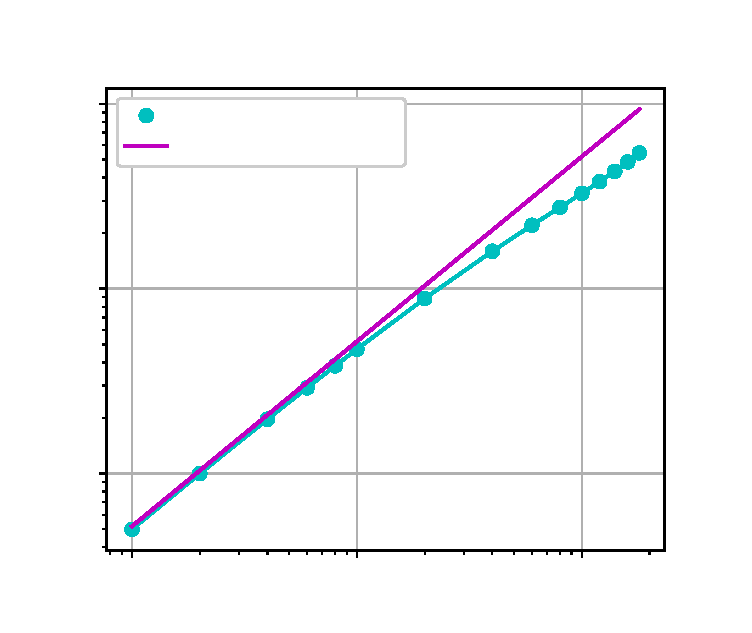
\includegraphics[width=\unitlength]{images_2ddl/lineaire.eps}}%
    \put(0.1257964,0.0485348){\color[rgb]{0,0,0}\makebox(0,0)[lb]{\smash{10}}}%
    \put(0.16297825,0.05963727){\color[rgb]{0,0,0}\makebox(0,0)[lb]{\smash{-2}}}%
    \put(0.43892111,0.04878857){\color[rgb]{0,0,0}\makebox(0,0)[lb]{\smash{10}}}%
    \put(0.47610296,0.05989104){\color[rgb]{0,0,0}\makebox(0,0)[lb]{\smash{-1}}}%
    \put(0.76074536,0.0485348){\color[rgb]{0,0,0}\makebox(0,0)[lb]{\smash{10}}}%
    \put(0.7979272,0.05963727){\color[rgb]{0,0,0}\makebox(0,0)[lb]{\smash{0}}}%
    \put(0.45736079,0.00605084){\color[rgb]{0,0,0}\makebox(0,0)[lb]{\smash{$\delta/R$ }}}%
    \put(0.05278422,0.18847651){\color[rgb]{0,0,0}\makebox(0,0)[lb]{\smash{10}}}%
    \put(0.08996607,0.19957897){\color[rgb]{0,0,0}\makebox(0,0)[lb]{\smash{2}}}%
    \put(0.05278422,0.44581787){\color[rgb]{0,0,0}\makebox(0,0)[lb]{\smash{10}}}%
    \put(0.08996607,0.45692033){\color[rgb]{0,0,0}\makebox(0,0)[lb]{\smash{3}}}%
    \put(0.05278422,0.70196636){\color[rgb]{0,0,0}\makebox(0,0)[lb]{\smash{10}}}%
    \put(0.08996607,0.71306882){\color[rgb]{0,0,0}\makebox(0,0)[lb]{\smash{4}}}%
    \put(0.03515632,0.373692){\color[rgb]{0,0,0}\rotatebox{90}{\makebox(0,0)[lb]{\smash{$F (N)$ }}}}%
    \put(0.23259861,0.68690835){\color[rgb]{0,0,0}\makebox(0,0)[lb]{\smash{étude éléments finis}}}%
    \put(0.23259861,0.64435615){\color[rgb]{0,0,0}\makebox(0,0)[lb]{\smash{théorie}}}%
  \end{picture}%
\endgroup%

\caption{Comparaison entre une étude éléments finis d'une roue en éléments poutres, dans laquelle on prend en compte les non linéarités géométriques, et le modèle théorique linéaire où la force appliquée et le déplacement sont liés par la constante $k$ selon la relation $F=k \delta$.}
\label{fig:lin1}
\end{figure}

La dérivation de la courbe de $F=f(\delta)$ obtenue par analyse éléments finis donne l'évolution de la raideur $k$ en fonction de $\delta/R$ (figure \ref{fig:lin2}).\\
Dans le domaine linéaire, on prendra comme valeur de $k$ la valeur moyenne des points situés dans la zone $\delta/R<0.1$

\begin{figure}[h]
\centering
%% Creator: Inkscape inkscape 0.92.2, www.inkscape.org
%% PDF/EPS/PS + LaTeX output extension by Johan Engelen, 2010
%% Accompanies image file 'lineaire2.eps' (pdf, eps, ps)
%%
%% To include the image in your LaTeX document, write
%%   \input{<filename>.pdf_tex}
%%  instead of
%%   \includegraphics{<filename>.pdf}
%% To scale the image, write
%%   \def\svgwidth{<desired width>}
%%   \input{<filename>.pdf_tex}
%%  instead of
%%   \includegraphics[width=<desired width>]{<filename>.pdf}
%%
%% Images with a different path to the parent latex file can
%% be accessed with the `import' package (which may need to be
%% installed) using
%%   \usepackage{import}
%% in the preamble, and then including the image with
%%   \import{<path to file>}{<filename>.pdf_tex}
%% Alternatively, one can specify
%%   \graphicspath{{<path to file>/}}
%% 
%% For more information, please see info/svg-inkscape on CTAN:
%%   http://tug.ctan.org/tex-archive/info/svg-inkscape
%%
\begingroup%
  \makeatletter%
  \providecommand\color[2][]{%
    \errmessage{(Inkscape) Color is used for the text in Inkscape, but the package 'color.sty' is not loaded}%
    \renewcommand\color[2][]{}%
  }%
  \providecommand\transparent[1]{%
    \errmessage{(Inkscape) Transparency is used (non-zero) for the text in Inkscape, but the package 'transparent.sty' is not loaded}%
    \renewcommand\transparent[1]{}%
  }%
  \providecommand\rotatebox[2]{#2}%
  \ifx\svgwidth\undefined%
    \setlength{\unitlength}{395.9999901bp}%
    \ifx\svgscale\undefined%
      \relax%
    \else%
      \setlength{\unitlength}{\unitlength * \real{\svgscale}}%
    \fi%
  \else%
    \setlength{\unitlength}{\svgwidth}%
  \fi%
  \global\let\svgwidth\undefined%
  \global\let\svgscale\undefined%
  \makeatother%
  \begin{picture}(1,0.833939)%
    \put(0,0){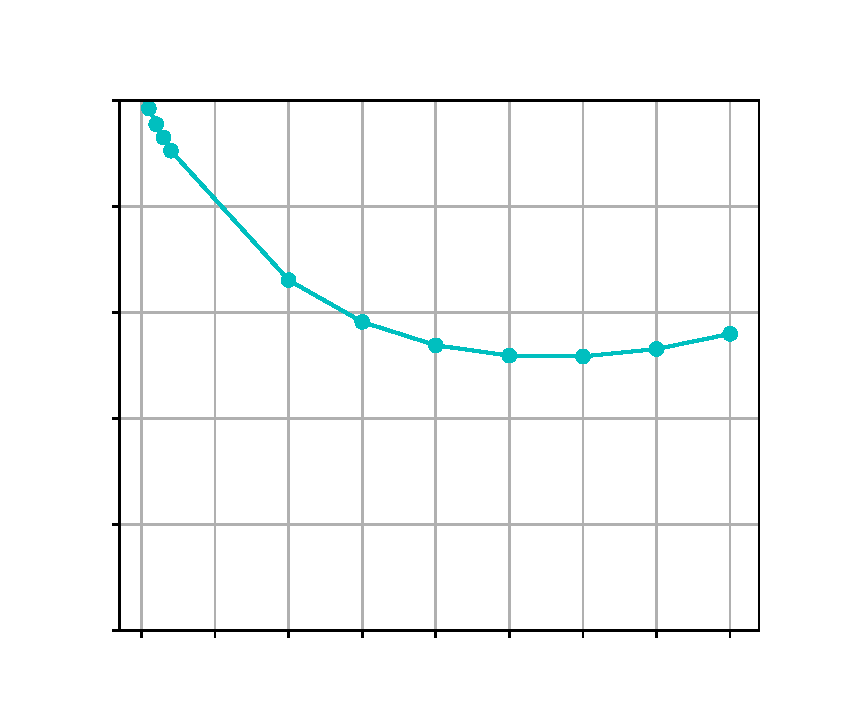
\includegraphics[width=\unitlength]{images_2ddl/lineaire2.eps}}%
    \put(0.13122525,0.05494683){\color[rgb]{0,0,0}\makebox(0,0)[lb]{\smash{0.0}}}%
    \put(0.22040808,0.05494683){\color[rgb]{0,0,0}\makebox(0,0)[lb]{\smash{0.2}}}%
    \put(0.30959091,0.05494683){\color[rgb]{0,0,0}\makebox(0,0)[lb]{\smash{0.4}}}%
    \put(0.39877273,0.05494683){\color[rgb]{0,0,0}\makebox(0,0)[lb]{\smash{0.6}}}%
    \put(0.48795707,0.05494683){\color[rgb]{0,0,0}\makebox(0,0)[lb]{\smash{0.8}}}%
    \put(0.57714141,0.05494683){\color[rgb]{0,0,0}\makebox(0,0)[lb]{\smash{1.0}}}%
    \put(0.66632323,0.05494683){\color[rgb]{0,0,0}\makebox(0,0)[lb]{\smash{1.2}}}%
    \put(0.75550505,0.05494683){\color[rgb]{0,0,0}\makebox(0,0)[lb]{\smash{1.4}}}%
    \put(0.84468939,0.05494683){\color[rgb]{0,0,0}\makebox(0,0)[lb]{\smash{1.6}}}%
    \put(0.09126414,0.08221173){\color[rgb]{0,0,0}\makebox(0,0)[lb]{\smash{0}}}%
    \put(0.04308712,0.21073142){\color[rgb]{0,0,0}\makebox(0,0)[lb]{\smash{1000}}}%
    \put(0.04308712,0.33925213){\color[rgb]{0,0,0}\makebox(0,0)[lb]{\smash{2000}}}%
    \put(0.04308712,0.46777233){\color[rgb]{0,0,0}\makebox(0,0)[lb]{\smash{3000}}}%
    \put(0.04308712,0.59629254){\color[rgb]{0,0,0}\makebox(0,0)[lb]{\smash{4000}}}%
    \put(0.04308712,0.72481274){\color[rgb]{0,0,0}\makebox(0,0)[lb]{\smash{5000}}}%
    \put(0.48795707,0.01){\color[rgb]{0,0,0}\makebox(0,0)[lb]{\smash{$\delta/R$ }}}%
    \put(0.02773838,0.36184557){\color[rgb]{0,0,0}\rotatebox{90}{\makebox(0,0)[lb]{\smash{$k$ $ (N \cdot m^{-1})$ }}}}%
  \end{picture}%
\endgroup%

\caption{Évolution du coefficient de raideur $k$ en fonction du ratio $\delta/R$. Cette courbe est obtenue par la dérivation des points de l'analyse éléments finis (figure \ref{fig:lin1}), en utilisant la méthode des différences finies centrées.}
\label{fig:lin2}
\end{figure}

\subsection{Mise en équations}

Les variables temporelles suivantes décrivent le mouvement du système comprimé puis relâché  (figure \ref{fig:saut}):

\begin{itemize}
    \item[$\bullet$] $t=-t_0$ : on relâche le ressort
    \item[$\bullet$] $t=0$ : la masse inférieure quitte le sol
    \item[$\bullet$] $t=t_f$ : le centre de gravité du système atteint sa hauteur maximale
\end{itemize}



\begin{figure}[h]

\def\svgwidth{400}
%% Creator: Inkscape inkscape 0.92.2, www.inkscape.org
%% PDF/EPS/PS + LaTeX output extension by Johan Engelen, 2010
%% Accompanies image file 'saut1.eps' (pdf, eps, ps)
%%
%% To include the image in your LaTeX document, write
%%   \input{<filename>.pdf_tex}
%%  instead of
%%   \includegraphics{<filename>.pdf}
%% To scale the image, write
%%   \def\svgwidth{<desired width>}
%%   \input{<filename>.pdf_tex}
%%  instead of
%%   \includegraphics[width=<desired width>]{<filename>.pdf}
%%
%% Images with a different path to the parent latex file can
%% be accessed with the `import' package (which may need to be
%% installed) using
%%   \usepackage{import}
%% in the preamble, and then including the image with
%%   \import{<path to file>}{<filename>.pdf_tex}
%% Alternatively, one can specify
%%   \graphicspath{{<path to file>/}}
%% 
%% For more information, please see info/svg-inkscape on CTAN:
%%   http://tug.ctan.org/tex-archive/info/svg-inkscape
%%
\begingroup%
  \makeatletter%
  \providecommand\color[2][]{%
    \errmessage{(Inkscape) Color is used for the text in Inkscape, but the package 'color.sty' is not loaded}%
    \renewcommand\color[2][]{}%
  }%
  \providecommand\transparent[1]{%
    \errmessage{(Inkscape) Transparency is used (non-zero) for the text in Inkscape, but the package 'transparent.sty' is not loaded}%
    \renewcommand\transparent[1]{}%
  }%
  \providecommand\rotatebox[2]{#2}%
  \ifx\svgwidth\undefined%
    \setlength{\unitlength}{458.93788937bp}%
    \ifx\svgscale\undefined%
      \relax%
    \else%
      \setlength{\unitlength}{\unitlength * \real{\svgscale}}%
    \fi%
  \else%
    \setlength{\unitlength}{\svgwidth}%
  \fi%
  \global\let\svgwidth\undefined%
  \global\let\svgscale\undefined%
  \makeatother%
  \begin{picture}(1,0.55996795)%
    \put(0,0){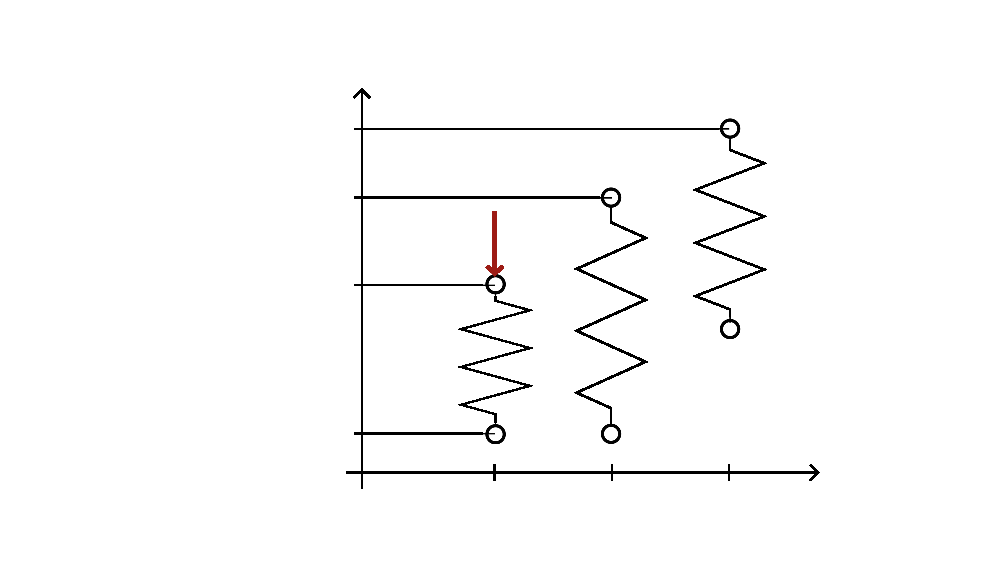
\includegraphics[width=\unitlength]{images_2ddl/saut1.eps}}%
    \put(0.35332121,0.50424636){\color[rgb]{0,0,0}\makebox(0,0)[lb]{\smash{$y$}}}%
    \put(0.85079889,0.07843695){\color[rgb]{0,0,0}\makebox(0,0)[lb]{\smash{$t$}}}%
    \put(0.44868441,0.03798154){\color[rgb]{0,0,0}\makebox(0,0)[lb]{\smash{$t<-t_0$}}}%
    \put(0.59510438,0.04003324){\color[rgb]{0,0,0}\makebox(0,0)[lb]{\smash{$t=0$}}}%
    \put(0.71660123,0.03978188){\color[rgb]{0,0,0}\makebox(0,0)[lb]{\smash{$t=t_f$}}}%
    \put(0.31206609,0.11596114){\color[rgb]{0,0,0}\makebox(0,0)[lb]{\smash{$0$}}}%
    \put(0.12576987,0.27218246){\color[rgb]{0,0,0}\makebox(0,0)[lb]{\smash{$2R-\dfrac{F}{k}-\dfrac{m_r g}{2k}$}}}%
    \put(0.19576987,0.36438468){\color[rgb]{0,0,0}\makebox(0,0)[lb]{\smash{$2R+\dfrac{m_r g}{2k}$}}}%
    \put(0.25429501,0.44056847){\color[rgb]{0,0,0}\makebox(0,0)[lb]{\smash{$y_{1,max}$}}}%
    \put(0.51238222,0.3284082){\color[rgb]{0.61568627,0.10588235,0.07843137}\makebox(0,0)[lb]{\smash{$F$}}}%
  \end{picture}%
\endgroup%


\caption{Saut du système. Pour $t<-t_0$, le système est écrasé par une force F. Il est relâché à $t=-t_0$, et la masse inférieure quitte le sol à $t=0$. Le centre de gravité du système atteint sa hauteur maximale pour $t=t_f$}
\label{fig:saut}
\end{figure}

Pour $-t_0<t<0$, la masse supérieure est soumise à deux forces verticales: son propre poids de norme $-m_r g/2$, et la force élastique de norme $-k(y_1-2R)$. Son mouvement est régi par:

\begin{equation}
    \frac{m_r}{2}\frac{d^2y_1}{dt^2}+k(y_1-2R)+\frac{m_r}{2}g=0,
  \label{eq:1}
\end{equation}

avec les condition initiales:
\begin{align}
    &y_1(-t_0)=2R-\frac{F}{k}-\frac{m_r g}{2k} \nonumber\\
    &\frac{dy_1}{dt}(-t_0)=0,
\label{eq:1i}
\end{align}

où $g$ est l'accélération gravitationnelle. \\
  
Pour $0<t<t_f$, la force que le ressort exerce sur la masse inférieure devient suffisante pour prendre le dessus sur la gravité: $m_r g/2=k(y_1-2R)$,  et le mouvement des deux masses est régi par:

\begin{align}
    \frac{m_r}{2}\frac{d^2y_1}{dt^2}+k(y_1-y_2-2R)+\frac{m_r}{2}g&=0 \nonumber\\
    \frac{m_r}{2}\frac{d^2y_2}{dt^2}+k(y_2-y_1+2R)+\frac{m_r}{2}g&=0,
  \label{eq:3}
\end{align}

avec les conditions initiales: 
\begin{align}
    y_1(0)=&2R+\frac{m_r g}{2k} & \frac{d y_1}{dt}(0)=&v_{10}\nonumber\\
    y_2(0)=&0 & \frac{d y2}{dt}(0)=&0
  \label{eq:4}
\end{align}    
    

\begin{figure}[htb]
\centering
\def\svgwidth{350}
%% Creator: Inkscape inkscape 0.92.2, www.inkscape.org
%% PDF/EPS/PS + LaTeX output extension by Johan Engelen, 2010
%% Accompanies image file 'sautp.eps' (pdf, eps, ps)
%%
%% To include the image in your LaTeX document, write
%%   \input{<filename>.pdf_tex}
%%  instead of
%%   \includegraphics{<filename>.pdf}
%% To scale the image, write
%%   \def\svgwidth{<desired width>}
%%   \input{<filename>.pdf_tex}
%%  instead of
%%   \includegraphics[width=<desired width>]{<filename>.pdf}
%%
%% Images with a different path to the parent latex file can
%% be accessed with the `import' package (which may need to be
%% installed) using
%%   \usepackage{import}
%% in the preamble, and then including the image with
%%   \import{<path to file>}{<filename>.pdf_tex}
%% Alternatively, one can specify
%%   \graphicspath{{<path to file>/}}
%% 
%% For more information, please see info/svg-inkscape on CTAN:
%%   http://tug.ctan.org/tex-archive/info/svg-inkscape
%%
\begingroup%
  \makeatletter%
  \providecommand\color[2][]{%
    \errmessage{(Inkscape) Color is used for the text in Inkscape, but the package 'color.sty' is not loaded}%
    \renewcommand\color[2][]{}%
  }%
  \providecommand\transparent[1]{%
    \errmessage{(Inkscape) Transparency is used (non-zero) for the text in Inkscape, but the package 'transparent.sty' is not loaded}%
    \renewcommand\transparent[1]{}%
  }%
  \providecommand\rotatebox[2]{#2}%
  \ifx\svgwidth\undefined%
    \setlength{\unitlength}{431.9999892bp}%
    \ifx\svgscale\undefined%
      \relax%
    \else%
      \setlength{\unitlength}{\unitlength * \real{\svgscale}}%
    \fi%
  \else%
    \setlength{\unitlength}{\svgwidth}%
  \fi%
  \global\let\svgwidth\undefined%
  \global\let\svgscale\undefined%
  \makeatother%
  \begin{picture}(1,0.83333334)%
    \put(0,0){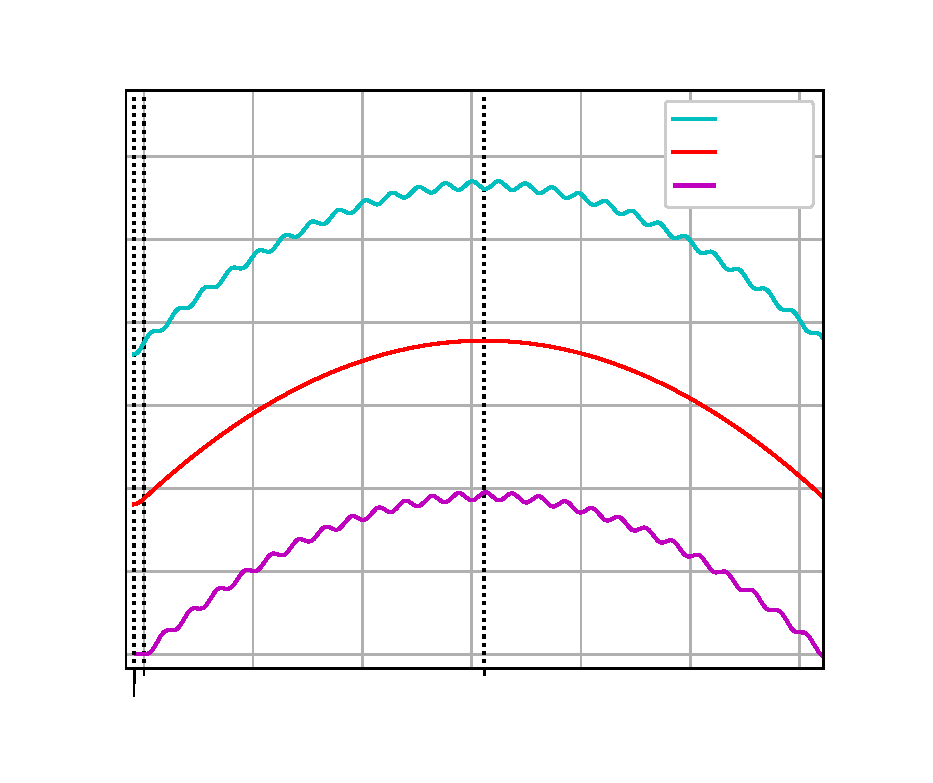
\includegraphics[width=\unitlength]{images_2ddl/sautp.eps}}%
    \put(0.79467593,0.71228239){\color[rgb]{0,0,0}\makebox(0,0)[lb]{\smash{$y_1(t)$}}}%
    \put(0.79467593,0.67524535){\color[rgb]{0,0,0}\makebox(0,0)[lb]{\smash{$y_{cdg}(t)$}}}%
    \put(0.79467593,0.63820832){\color[rgb]{0,0,0}\makebox(0,0)[lb]{\smash{$y_2(t)$}}}%
    \put(0.09341219,0.0388418){\color[rgb]{0,0,0}\makebox(0,0)[lb]{\smash{$-t_0$}}}%
    \put(0.135556003,0.06552941){\color[rgb]{0,0,0}\makebox(0,0)[lb]{\smash{$0$}}}%
    \put(0.5175824,0.06311792){\color[rgb]{0,0,0}\makebox(0,0)[lb]{\smash{$t_f$}}}%
    \put(0.05446337,0.76775099){\color[rgb]{0,0,0}\makebox(0,0)[lb]{\smash{$y (m)$}}}%
    \put(0.86146302,0.06058865){\color[rgb]{0,0,0}\makebox(0,0)[lb]{\smash{$t (s)$}}}%
  \end{picture}%
\endgroup%


\caption{Évolution temporelle des positions des masses et du centre de gravité lors du saut du système}
\label{fig:saut}
\end{figure}

Avant de résoudre le problème, on le réécrit sous forme adimensionnelle:
on définit le temps adimensionnel $\tau=t\sqrt{\dfrac{2k}{m_r}}$ et les variables positions adimensionnelles $\xi_1=y_1 \dfrac{2k}{m_r g}$ et $\xi_2=y_2 \dfrac{2k}{m_r g}$ \\

 L'équation \ref{eq:1} devient:
\begin{equation}
    \frac{d^2\xi_1}{d\tau^2}+\xi_1-\xi_0+1=0,
  \label{eq:1a}
\end{equation}
\\
pour $-\tau_0<\tau<0$,\\
avec $\xi_0=\dfrac{4Rk}{m_r g}$ et $\tau_0=t_0 \sqrt{\frac{2k}{m_r}}$ \\

et avec les conditions initiales
\begin{align}
    &\xi_1(-\tau_0)=\xi_0-\frac{2F}{m_r g}-1 \nonumber\\
    &\frac{d\xi_1}{d\tau}(-\tau_0)=0
\label{eq:1ia}
\end{align}
 

De même, l'équation \ref{eq:3} devient:
\begin{align}
    \frac{d^2\xi_1}{d\tau^2}+\xi_1-\xi_2-\xi_0+1&=0 \nonumber\\
    \frac{d^2\xi_2}{d\tau^2}+\xi_2-\xi_1+\xi_0+1&=0
  \label{eq:3a}
\end{align}

pour $0<\tau<\tau_f$,\\
avec $\tau_f=t_f \sqrt{\frac{2k}{m_r}}$ \\
et avec les conditions initiales: 
\begin{align}
    \xi_1(0)&=\xi_0+1   &  \frac{d xi_1}{d\tau}(0)&=\zeta_{10} \nonumber\\
    \xi_2(0)&=0   &  \frac{d \xi_2}{d\tau}(0)&=0
  \label{eq:4a}
\end{align} 

En résolvant \ref{eq:1a} avec les conditions initiales \ref{eq:1ia}, on obtient l'équation du mouvement \ref{eq:2} pour $-\tau_0<\tau<0$:
\begin{align}
    \xi_1&=-frac{-2F}{m_r g}(\cos{-\tau_0}\cos{\tau}+\sin{-\tau_0}\sin{\tau})+\xi_0-1 \nonumber\\
    \xi_2&=0
  \label{eq:2}
\end{align}

En résolvant \ref{eq:3a} avec les conditions initiales \ref{eq:4a}, on obtient l'équation du mouvement \ref{eq:5a} pour $0<\tau<\tau_f$:
\begin{align}
    \xi_1&=-\frac{1}{2}\tau^2+\frac{\zeta_{10}}{2}\tau+\frac{\zeta_{10}}{2\sqrt{2}}\sin{(\sqrt{2}\tau)}+\frac{1}{2}\cos{(\sqrt{2}\tau)}+\xi_0+\frac{1}{2} \nonumber\\
    \xi_2&=-\frac{1}{2}\tau^2+\frac{\zeta_{10}}{2}\tau-\frac{\zeta_{10}}{2\sqrt{2}}\sin{(\sqrt{2}\tau)}-\frac{1}{2}\cos{(\sqrt{2}\tau)}-\frac{1}{2}
  \label{eq:5a}
\end{align}

La vitesse initiale adimensionnelle de la masse supérieure s'exprime
\begin{equation}
    \zeta_{10}=\frac{d\xi_1}{d\tau}(0)=-\frac{2F}{m_r g}\sin{-\tau_0}
    \label{eq:c1}
\end{equation}


D'après les conditions initiales \ref{eq:4a} appliquées à l'équation \ref{eq:2}, on a par continuité:
\begin{equation}
    \cos{-\tau_0}=-\frac{m_r g}{F}
    \label{eq:c2}
\end{equation}

On substitue \ref{eq:c2} à l'intérieur de \ref{eq:c1}:
\begin{equation}
    \zeta_{10}=\sqrt{(\frac{2F}{m_r g})^2-4}
    \label{eq:c3}
\end{equation}

La positon adimensionnelle du centre de gravité du système s'écrit $\xi_{cdg}(\tau)=\dfrac{\xi_1(\tau)+\xi_2(\tau)}{2}$. En substituant \ref{eq:5a} dans cette expression, on obtient: 

\begin{equation}
  \xi_{cdg}(\tau)=-\frac{1}{2}\tau^2+\frac{\zeta_{10}}{2}\tau+\frac{\xi_0+1}{2}
  \label{eq:cdg}
\end{equation}

En substituant \ref{eq:c3} dans \ref{eq:cdg} on obtient:

\begin{equation}
  \xi_{cdg}(\tau)=-\frac{1}{2}\tau^2+\sqrt{(\frac{F}{m_r g})^2-1}\tau+\frac{\xi_0+1}{2}
  \label{eq:cdg2}
\end{equation}

Durant l'élévation du centre de gravité de la roue, on observe des déformations correspondant au second mode vibratoire d'un anneau (déformations planes).

Lorsqu'on arrive à $\tau=\tau_f$, la vitesse du centre de gravité s'annule. En dérivant \ref{eq:cdg2}, on trouve l'expression de $\tau_f$:

\begin{equation}
    \tau_f=\sqrt{(\frac{F}{m_r g})^2-1}
    \label{eq:tauf}
\end{equation}

On substitue ensuite \ref{eq:tauf} à l'intérieur de \ref{eq:cdg2} pour obtenir l'expression de la hauteur maximale du centre de gravité:

\begin{equation}
  \xi_{cdg,max}=\frac{1}{2}((\frac{F}{m_r g})^2-1)+\frac{\xi_0+1}{2}
  \label{eq:cdgmax}
\end{equation}

On soustrait ensuite à \ref{eq:cdgmax} sa position adimensionnelle à l'équilibre statique $\xi_{cdg,ref}=\dfrac{\xi_0-1}{2}$ pour obtenir l'expression adimensionnelle $\eta_{max}=\dfrac{2k}{m_rg}H_{max}$:


\begin{equation}
\eta_{max}=\frac{1}{2}((\frac{F}{m_r g})^2+1)
 \label{eq:hmax}
\end{equation}


Ainsi, les paramètres influençant la hauteur maximale de saut du système sont:
\begin{itemize}
    \item La force de compression $F$ à laquelle ce dernier est soumis initialement
    \item La masse du système, déterminée par sa géométrie et la masse volumique du matériau
    \item La raideur équivalente du système qui dépend de sa géométrie et du module de Young du matériau.
\end{itemize}

L'expression de $H_{max}$ permet d'étudier l'efficacité énergétique du système, c'est à dire la fraction de l'énergie totale $E_{tot}$ fournie au système sous forme de déformation élastique qui est convertie en énergie potentielle gravitationnelle $E_{p,g}$ servant au saut. \\
Avec $E_{tot}=\dfrac{F^2}{2k}$ et $E_{p,g}=m_r g H_{max}$,\\
L'efficacité énergétique s'exprime:  $\dfrac{E_{p,g}}{E_{tot}}=\dfrac{1}{2}((\dfrac{m_r g}{F})^2+1)$.

\subsection{Valeurs limites et premiers résultats}
Dans la partie qui suit, on étudie les variations de $\eta_{max}$, la hauteur maximale de saut adimensionnelle et du ratio d'efficacité énergétique.
\\ 
\\ 
Les paramètres $F$, $k$ et $m_r$ doivent rester supérieurs aux valeurs limites suivantes, en dessous desquelles le modèle n'est plus valide:
\begin{itemize}
    \item Pour $F$: l'énergie de déformation élastique doit être suffisante pour faire décoller le système, ce qui se traduit par: $F/m_r g>1$
    \item Pour $k$: le ressort doit pouvoir soutenir la masse 1: $m_r g/2k<2R$ c'est à dire: $k>m_r g/4R$ 
    \item Pour $m_r$: diminuer $m_r$ revient à retirer de la matière, il y a donc une masse limite dépendant des propriétés mécaniques du matériau en dessous de laquelle il y aura endommagement lors de l'utilisation, la roue étant devenue trop fragile.
\end{itemize}
Ces limites seront indiquées par des pointillés sur les tracés des figures \ref{fig:eta} et \ref{fig:effe}.
\\

\begin{figure}[htb]
\centering
\def\svgwidth{320}
%% Creator: Inkscape inkscape 0.92.2, www.inkscape.org
%% PDF/EPS/PS + LaTeX output extension by Johan Engelen, 2010
%% Accompanies image file 'eta.eps' (pdf, eps, ps)
%%
%% To include the image in your LaTeX document, write
%%   \input{<filename>.pdf_tex}
%%  instead of
%%   \includegraphics{<filename>.pdf}
%% To scale the image, write
%%   \def\svgwidth{<desired width>}
%%   \input{<filename>.pdf_tex}
%%  instead of
%%   \includegraphics[width=<desired width>]{<filename>.pdf}
%%
%% Images with a different path to the parent latex file can
%% be accessed with the `import' package (which may need to be
%% installed) using
%%   \usepackage{import}
%% in the preamble, and then including the image with
%%   \import{<path to file>}{<filename>.pdf_tex}
%% Alternatively, one can specify
%%   \graphicspath{{<path to file>/}}
%% 
%% For more information, please see info/svg-inkscape on CTAN:
%%   http://tug.ctan.org/tex-archive/info/svg-inkscape
%%
\begingroup%
  \makeatletter%
  \providecommand\color[2][]{%
    \errmessage{(Inkscape) Color is used for the text in Inkscape, but the package 'color.sty' is not loaded}%
    \renewcommand\color[2][]{}%
  }%
  \providecommand\transparent[1]{%
    \errmessage{(Inkscape) Transparency is used (non-zero) for the text in Inkscape, but the package 'transparent.sty' is not loaded}%
    \renewcommand\transparent[1]{}%
  }%
  \providecommand\rotatebox[2]{#2}%
  \ifx\svgwidth\undefined%
    \setlength{\unitlength}{344.79999138bp}%
    \ifx\svgscale\undefined%
      \relax%
    \else%
      \setlength{\unitlength}{\unitlength * \real{\svgscale}}%
    \fi%
  \else%
    \setlength{\unitlength}{\svgwidth}%
  \fi%
  \global\let\svgwidth\undefined%
  \global\let\svgscale\undefined%
  \makeatother%
  \begin{picture}(1,0.83526682)%
    \put(0,0){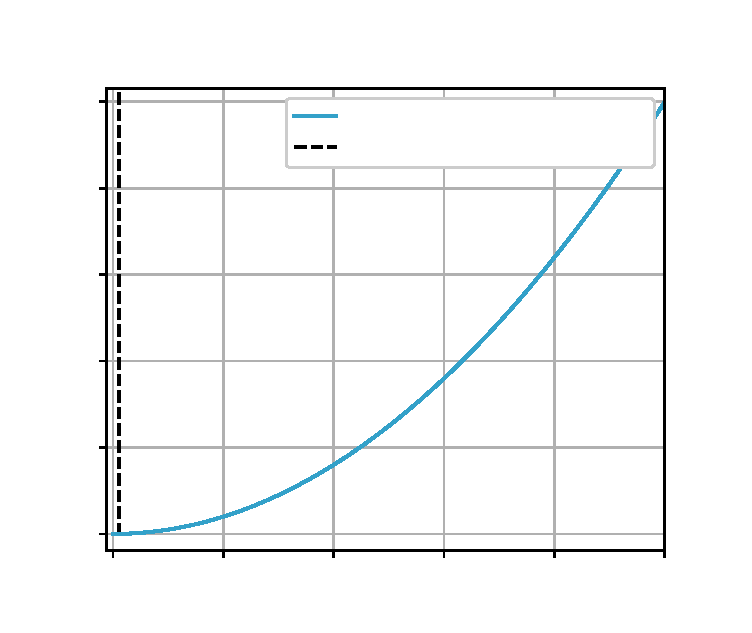
\includegraphics[width=\unitlength]{images_2ddl/eta.eps}}%
    \put(0.12494664,0.04955423){\color[rgb]{0,0,0}\makebox(0,0)[lb]{\smash{0}}}%
    \put(0.26935006,0.04955423){\color[rgb]{0,0,0}\makebox(0,0)[lb]{\smash{20}}}%
    \put(0.42297564,0.04955423){\color[rgb]{0,0,0}\makebox(0,0)[lb]{\smash{40}}}%
    \put(0.57660093,0.04955423){\color[rgb]{0,0,0}\makebox(0,0)[lb]{\smash{60}}}%
    \put(0.73022622,0.04955423){\color[rgb]{0,0,0}\makebox(0,0)[lb]{\smash{80}}}%
    \put(0.87462877,0.04955423){\color[rgb]{0,0,0}\makebox(0,0)[lb]{\smash{100}}}%
    \put(0.08654466,0.10358121){\color[rgb]{0,0,0}\makebox(0,0)[lb]{\smash{0}}}%
    \put(0.03121375,0.22391821){\color[rgb]{0,0,0}\makebox(0,0)[lb]{\smash{1000}}}%
    \put(0.03121375,0.34425464){\color[rgb]{0,0,0}\makebox(0,0)[lb]{\smash{2000}}}%
    \put(0.03121375,0.46459107){\color[rgb]{0,0,0}\makebox(0,0)[lb]{\smash{3000}}}%
    \put(0.03121375,0.58492749){\color[rgb]{0,0,0}\makebox(0,0)[lb]{\smash{4000}}}%
    \put(0.03121375,0.70526392){\color[rgb]{0,0,0}\makebox(0,0)[lb]{\smash{5000}}}%
    \put(0.46800464,0.68690835){\color[rgb]{0,0,0}\makebox(0,0)[lb]{\smash{$\eta_{max}$}}}%
    \put(0.46800464,0.64354118){\color[rgb]{0,0,0}\makebox(0,0)[lb]{\smash{\small valeur minimale de  $F/m_r g$ }}}%
    \put(0.46,0.0155423){\color[rgb]{0,0,0}\makebox(0,0)[lb]{\smash{$F/m_r g$}}}%
  \end{picture}%
\endgroup%

\caption{Variation de la hauteur maximale de saut adimensionnelle $\eta_{max}$ en fonction du ratio $F/m_r g$}
\label{fig:eta}
\end{figure}

\begin{figure}[htb]
\centering
\def\svgwidth{320}
%% Creator: Inkscape inkscape 0.92.2, www.inkscape.org
%% PDF/EPS/PS + LaTeX output extension by Johan Engelen, 2010
%% Accompanies image file 'eff.eps' (pdf, eps, ps)
%%
%% To include the image in your LaTeX document, write
%%   \input{<filename>.pdf_tex}
%%  instead of
%%   \includegraphics{<filename>.pdf}
%% To scale the image, write
%%   \def\svgwidth{<desired width>}
%%   \input{<filename>.pdf_tex}
%%  instead of
%%   \includegraphics[width=<desired width>]{<filename>.pdf}
%%
%% Images with a different path to the parent latex file can
%% be accessed with the `import' package (which may need to be
%% installed) using
%%   \usepackage{import}
%% in the preamble, and then including the image with
%%   \import{<path to file>}{<filename>.pdf_tex}
%% Alternatively, one can specify
%%   \graphicspath{{<path to file>/}}
%% 
%% For more information, please see info/svg-inkscape on CTAN:
%%   http://tug.ctan.org/tex-archive/info/svg-inkscape
%%
\begingroup%
  \makeatletter%
  \providecommand\color[2][]{%
    \errmessage{(Inkscape) Color is used for the text in Inkscape, but the package 'color.sty' is not loaded}%
    \renewcommand\color[2][]{}%
  }%
  \providecommand\transparent[1]{%
    \errmessage{(Inkscape) Transparency is used (non-zero) for the text in Inkscape, but the package 'transparent.sty' is not loaded}%
    \renewcommand\transparent[1]{}%
  }%
  \providecommand\rotatebox[2]{#2}%
  \ifx\svgwidth\undefined%
    \setlength{\unitlength}{344.79999138bp}%
    \ifx\svgscale\undefined%
      \relax%
    \else%
      \setlength{\unitlength}{\unitlength * \real{\svgscale}}%
    \fi%
  \else%
    \setlength{\unitlength}{\svgwidth}%
  \fi%
  \global\let\svgwidth\undefined%
  \global\let\svgscale\undefined%
  \makeatother%
  \begin{picture}(1,0.83526682)%
    \put(0,0){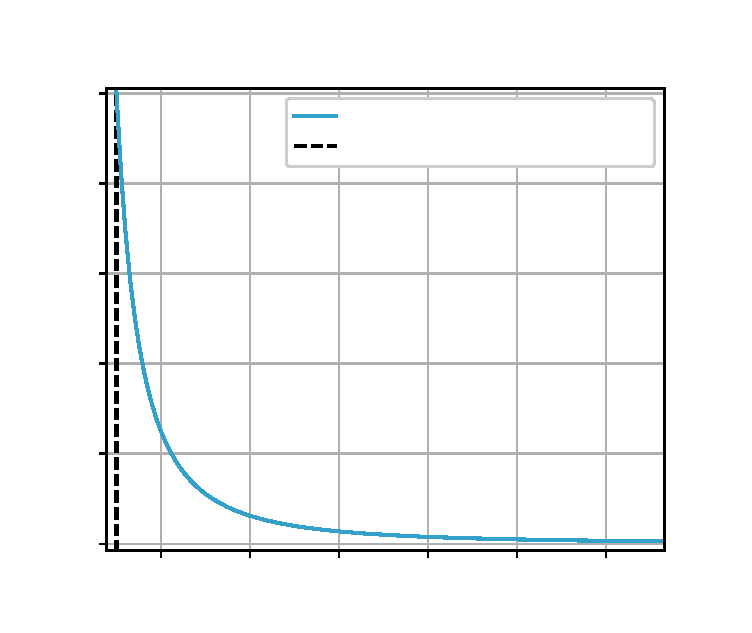
\includegraphics[width=\unitlength]{images_2ddl/eff.eps}}%
    \put(0.19169287,0.04955423){\color[rgb]{0,0,0}\makebox(0,0)[lb]{\smash{2}}}%
    \put(0.31560035,0.04955423){\color[rgb]{0,0,0}\makebox(0,0)[lb]{\smash{4}}}%
    \put(0.43950406,0.04955423){\color[rgb]{0,0,0}\makebox(0,0)[lb]{\smash{6}}}%
    \put(0.56341067,0.04955423){\color[rgb]{0,0,0}\makebox(0,0)[lb]{\smash{8}}}%
    \put(0.67809745,0.04955423){\color[rgb]{0,0,0}\makebox(0,0)[lb]{\smash{10}}}%
    \put(0.80200116,0.04955423){\color[rgb]{0,0,0}\makebox(0,0)[lb]{\smash{12}}}%
    \put(0.05885673,0.08975435){\color[rgb]{0,0,0}\makebox(0,0)[lb]{\smash{0.5}}}%
    \put(0.05885673,0.21525174){\color[rgb]{0,0,0}\makebox(0,0)[lb]{\smash{0.6}}}%
    \put(0.05885673,0.34074826){\color[rgb]{0,0,0}\makebox(0,0)[lb]{\smash{0.7}}}%
    \put(0.05885673,0.4662471){\color[rgb]{0,0,0}\makebox(0,0)[lb]{\smash{0.8}}}%
    \put(0.05885673,0.59174304){\color[rgb]{0,0,0}\makebox(0,0)[lb]{\smash{0.9}}}%
    \put(0.05885673,0.71724188){\color[rgb]{0,0,0}\makebox(0,0)[lb]{\smash{1.0}}}%
    \put(0.46800464,0.68690835){\color[rgb]{0,0,0}\makebox(0,0)[lb]{\smash{$E_{p,g}/E_{tot}$}}}%
    \put(0.46800464,0.64435615){\color[rgb]{0,0,0}\makebox(0,0)[lb]{\smash{\small valeur minimale de $F/m_r g$ }}}%
    \put(0.460200116,0.0155423){\color[rgb]{0,0,0}\makebox(0,0)[lb]{\smash{$F/m_r g$}}}%
  \end{picture}%
\endgroup%

\caption{Variation de l'efficacité énergétique en fonction du ratio $\dfrac{F}{m_r g}$}
\label{fig:effe}
\end{figure}

Remarques:

\begin{itemize}
    \item Les tracés adimensionnels permettent d'étudier une tendance globale, en s'affranchissant de la dépendance des résultats avec les autres paramètres.
    \item On identifie deux modes pour le mouvement du système: le mode de translation caractérisé par l'évolution de la position du centre de gravité donnée à l'équation \ref{eq:cdg2}
    $$\xi_{translation}(\tau)=-\frac{1}{2}\tau^2+\sqrt{(\frac{F}{m_r g})^2-1}\tau+\frac{2Rk}{m_r g}+\frac{1}{2},$$ et le mode de vibration, obtenu par la soustraction des positions des deux masses données dans l'équation \ref{eq:5a}: 
    $$\xi_{vibration}=\frac{\xi_1 - \xi_2}{2},$$ soit $$\xi_{vibration}=\frac{1}{2\sqrt{2}}\sin{(\sqrt{2}\tau)}\sqrt{(\frac{2F}{m_r g})^2-4}+\frac{1}{2}\cos{(\sqrt{2}\tau)}+\frac{2Rk}{m_r g}+\frac{1}{2}.$$
    Ces expressions illustrent ce qu'on constate en observant les figures \ref{fig:eta} et \ref{fig:effe}: plus le ratio $\dfrac{F}{m_r g}$ est important, plus les amplitudes des modes de translation et de vibration augmentent, et donc la hauteur maximale de saut $H_{max}$ et l'amplitude des vibrations augmentent toutes les deux. Ainsi l'efficacité énergétique décroît car l'énergie dissipée par vibration augmente en même temps que $H_{max}$ avec le ratio $\dfrac{F}{m_r g}$.
\end{itemize}

\subsection{Mise en évidence de différents régimes de saut}
Les résultats et conclusions des sous-sections précédentes sont synthétisés en figure \ref{fig:regime}. On différencie d'une part le régime linéaire du régime non linéaire selon la valeur du ratio $\delta/R$, où $\delta$ est la flèche imposée par la force $F$. On rappelle que la valeur limite en comportement linéaire a été fixée à $\delta/R=0.1$. Il existe également trois régimes de saut distincts, en fonction du ratio $\dfrac{F}{m_r g}$. Le premier, trivial, correspond au cas où la force appliquée ne suffit pas à soulever la roue: il n'y a pas de saut. Le passage d'un saut efficace énergétiquement à un saut peu efficace est déterminée par la dissipation d'énergie par vibration: plus la force augmente par rapport au poids de la roue, plus l'amplitude du mode de vibration augmente, et plus l'efficacité énergétique du saut décroît.


\begin{figure}[htb]
\def\svgwidth{400}
%% Creator: Inkscape inkscape 0.92.2, www.inkscape.org
%% PDF/EPS/PS + LaTeX output extension by Johan Engelen, 2010
%% Accompanies image file 'regimes1.eps' (pdf, eps, ps)
%%
%% To include the image in your LaTeX document, write
%%   \input{<filename>.pdf_tex}
%%  instead of
%%   \includegraphics{<filename>.pdf}
%% To scale the image, write
%%   \def\svgwidth{<desired width>}
%%   \input{<filename>.pdf_tex}
%%  instead of
%%   \includegraphics[width=<desired width>]{<filename>.pdf}
%%
%% Images with a different path to the parent latex file can
%% be accessed with the `import' package (which may need to be
%% installed) using
%%   \usepackage{import}
%% in the preamble, and then including the image with
%%   \import{<path to file>}{<filename>.pdf_tex}
%% Alternatively, one can specify
%%   \graphicspath{{<path to file>/}}
%% 
%% For more information, please see info/svg-inkscape on CTAN:
%%   http://tug.ctan.org/tex-archive/info/svg-inkscape
%%
\begingroup%
  \makeatletter%
  \providecommand\color[2][]{%
    \errmessage{(Inkscape) Color is used for the text in Inkscape, but the package 'color.sty' is not loaded}%
    \renewcommand\color[2][]{}%
  }%
  \providecommand\transparent[1]{%
    \errmessage{(Inkscape) Transparency is used (non-zero) for the text in Inkscape, but the package 'transparent.sty' is not loaded}%
    \renewcommand\transparent[1]{}%
  }%
  \providecommand\rotatebox[2]{#2}%
  \ifx\svgwidth\undefined%
    \setlength{\unitlength}{556.9991112bp}%
    \ifx\svgscale\undefined%
      \relax%
    \else%
      \setlength{\unitlength}{\unitlength * \real{\svgscale}}%
    \fi%
  \else%
    \setlength{\unitlength}{\svgwidth}%
  \fi%
  \global\let\svgwidth\undefined%
  \global\let\svgscale\undefined%
  \makeatother%
  \begin{picture}(1,0.59015529)%
    \put(0,0){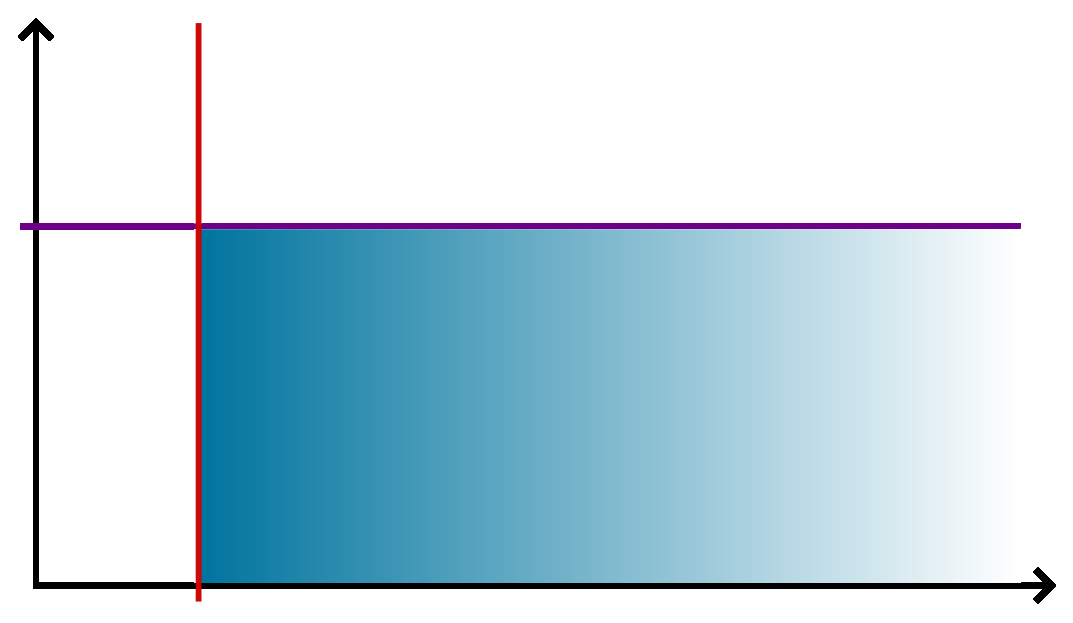
\includegraphics[width=\unitlength]{images_2ddl/regimes1.eps}}%
    \put(0.02561396,0.28811823){\color[rgb]{0,0,0}\makebox(0,0)[lb]{\smash{}}}%
    \put(0.066009,0.05921302){\color[rgb]{0,0,0}\makebox(0,0)[lb]{\smash{}}}%
    \put(-0.01,0.0){\color[rgb]{0,0,0}\makebox(0,0)[lb]{\smash{0}}}%
    \put(-0.0384028,0.35794642){\color[rgb]{0,0,0}\makebox(0,0)[lb]{\smash{0.1}}}%
    \put(0.170346148,-0.02){\color[rgb]{0,0,0}\makebox(0,0)[lb]{\smash{1}}}%
    \put(0.095137172,0.25955463){\color[rgb]{0.8,0,0}\makebox(0,0)[b]{\smash{PAS}}}%
    \put(0.095137172,0.20955463){\color[rgb]{0.8,0,0}\makebox(0,0)[b]{\smash{DE}}}%
    \put(0.095137172,0.15955463){\color[rgb]{0.8,0,0}\makebox(0,0)[b]{\smash{SAUT}}}%
    \put(0.350802717,0.23077807){\color[rgb]{0,0,0.01176471}\makebox(0,0)[b]{\smash{SAUT AVEC PEU}}}%
    \put(0.350802717,0.18077807){\color[rgb]{0,0,0.01176471}\makebox(0,0)[b]{\smash{DE VIBRATIONS}}}%
    \put(0.75539718,0.20955463){\color[rgb]{0,0,0.02745098}\makebox(0,0)[b]{\smash{SAUT  EFFICACE À 50\%}}}%
    \put(0.22758915,0.44969837){\color[rgb]{0,0,0}\makebox(0,0)[lb]{\smash{}}}%
    \put(0.58988013,0.43773024){\color[rgb]{0.43137255,0,0.53333333}\makebox(0,0)[b]{\smash{NON LINÉARITÉ GÉOMÉTRIQUE}}}%
    \put(0.0,0.59741848){\color[rgb]{0,0,0}\makebox(0,0)[lb]{\smash{$\dfrac{F}{kR}$}}}%
    \put(0.96816481,0.05921302){\color[rgb]{0,0,0}\makebox(0,0)[lb]{\smash{}}}%
    \put(1.01,0.01016188){\color[rgb]{0,0,0}\makebox(0,0)[lb]{\smash{$\dfrac{F}{m_r g}$}}}%
  \end{picture}%
\endgroup%

\caption{Carte des différents régimes de saut possibles pour une roue Cyr en fonction des ratios $F/kR$ et $F/m_r g$.}
\label{fig:regime}
\end{figure}

\subsection{Étude de $H_{max}$ en fonction de la géométrie de la section}
Nous avons vu que la rigidité $k$ et la masse $m_r$ de la roue sont des paramètres déterminants pour $H_{max}$. 
D'après \ref{eq:km1}, on peut moduler $k$ et $m_r$ en jouant sur les propriétés du matériau avec la masse volumique $\rho$ et le module de Young $E$, ou bien en jouant sur la géométrie avec le rayon médian de la roue $R$ et les rayons intérieur et extérieur de la section $r_1$, $r_2$ qui déterminent l'aire de section $A$ et le moment quadratique de section $I$.
\begin{align}
    k&=\frac{4\pi EI}{(\pi^2 -8)R^3} &  I&=\frac{\pi}{4}(r_2^4-r_1^4) \nonumber\\
    m_r&=2\pi R \rho A   & A&=\pi (r_2^2-r_1^2)
    \label{eq:km1}
\end{align}

Les dimensions de la section, caractérisées par $r_1$ et $r_2$, sont les paramètres les plus malléables. Nous allons étudier leur influence sur la hauteur maximale de saut puis en déduire des valeurs optimisées. \\
Le matériau considéré dans cette étude sera le matériau ayant le module de Young le plus élevé parmi ceux disponibles pour l'imprimante 3D utilisée.\\
Il s'agit du nylon renforcé avec des fibres de carbone courtes, ayant pour masse volumique $\rho=1170 kg \cdot m^{-3}$, pour module d'Young $E=9.0 GPa$, pour module de cisaillement $G=3.8 GPa$ et une contrainte à la rupture $\sigma_r=63.0 MPa$.\\
Le rayon médian $R$ de la roue sera compris entre $0.8 m$ et $1.0 m$, nous fixons sa valeur à $0.9 m$. \\
On considère deux types de chargement pour la force de compression $F$ appliquée au sommet de la roue: 
\begin{itemize}
    \item $F_1=900 N$, qui correspond au cas où l'utilisateur se suspend par une main à la roue, la charge maximum qu'il peut appliquer en statique. 
    \item $F_2=c_d F_1 $, où $c_d=5$ rend compte des effets dynamiques. Le choix de la valeur de $c_d$ est basé sur des articles traitant des efforts dynamiques à l'impact exercés par des gymnastes lors de mouvements acrobatiques \cite{marinsek},\cite{seegmiller_ground_nodate}, \cite{mcnair_normative_1999},\cite{prapavessis_effects_1999} et sur les travaux de Marion Cossin, mesurant les efforts exercés par des circassiens suspendus à des agrès aériens \cite{cossin_mesure_nodate}.
\end{itemize}
 

$H_{max}$ décroît avec $k$ et $m_r$ selon les lois modélisées dans les sections précédentes. Maximiser $H_{max}$ en jouant sur les paramètres $r_1$ et $r_2$ revient à minimiser les valeurs de $I$ et de $A$, et donc réduire l'épaisseur de section. \\
La première étape qui s'impose est de définir des limites inférieures de l'épaisseur de section pour s'assurer que la roue ne sera ni sujette à du flambement, de l'écoulement et qu'on restera dans le domaine de comportement linéaire.
Dans ce qui suit pour chaque valeur fixe du rayon externe $r_2$, comprise entre $10 mm$ et $50 mm$, nous étudierons le comportement de la roue pour un rayon interne $r_1$ variant de $0 mm$ à $r_2 - 0.01 mm$.

\subsubsection{Limites en flambement et en écoulement lors de la compression}

Lorsqu'on exerce une force de compression au sommet de la roue, des phénomènes de flambement et d'écoulement apparaissent si sa section n'est pas assez épaisse. 
Pour chaque valeur du rayon externe $r_2$, compris entre $10 mm$ et $50 mm$, on cherche à savoir quelle est la valeur maximale du rayon interne $r_1$ permettant d'éviter ces phénomènes. 

 \begin{figure}[h]
\centering
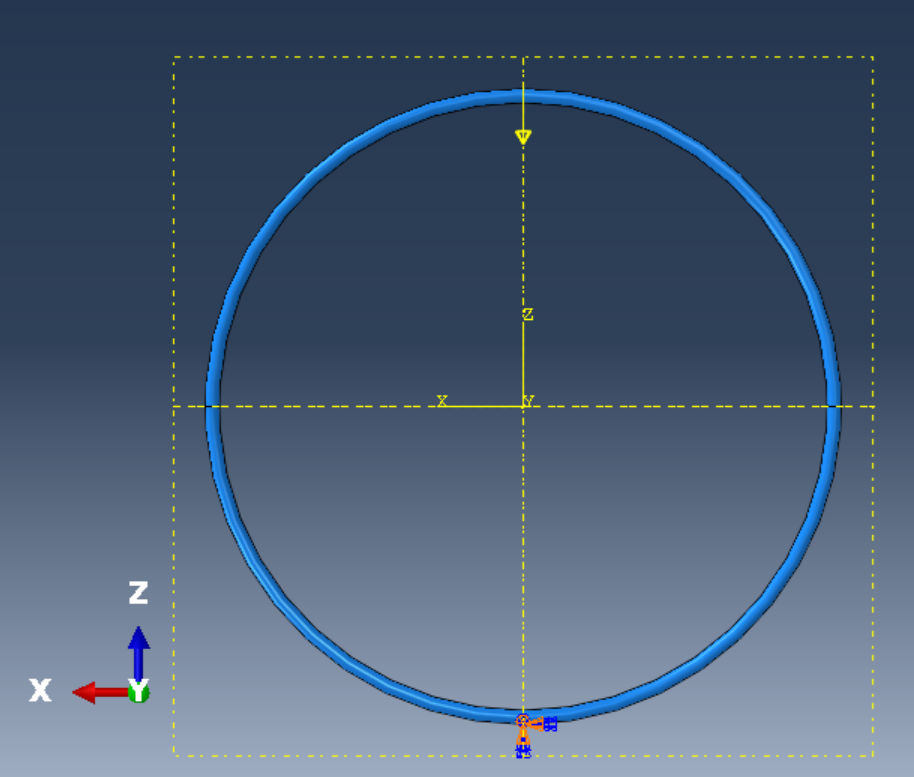
\includegraphics[width=200]{saut2/elf1.PNG}
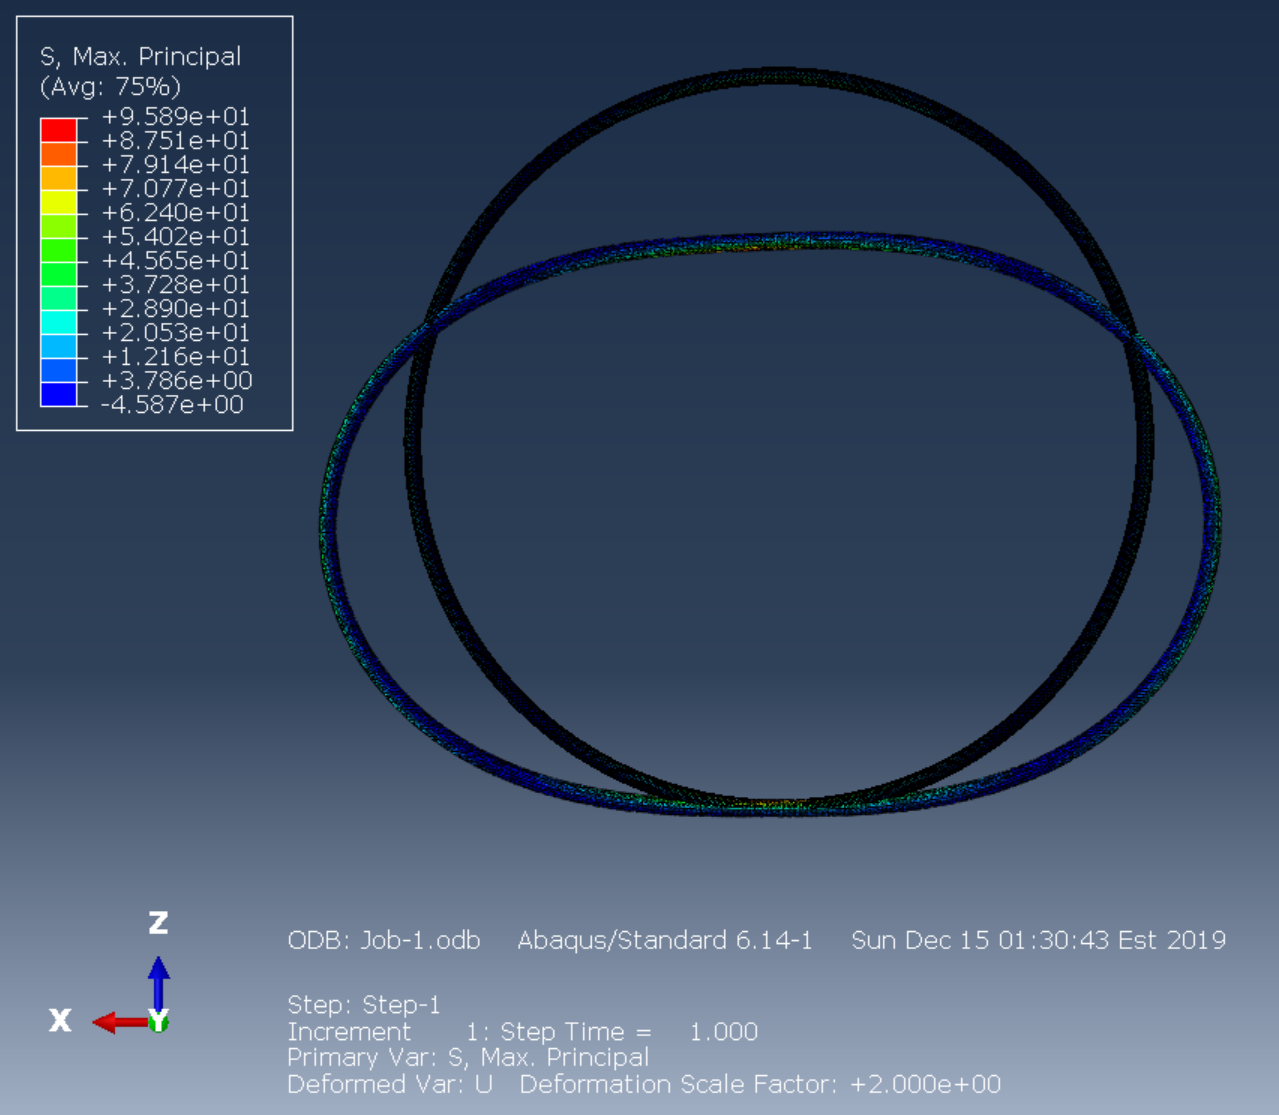
\includegraphics[width=241]{saut2/elf2.PNG}
\caption{Modélisation éléments finis d'une roue Cyr comprimée par une force exercée à son sommet.}
\label{fig:elf1}
\end{figure}

Pour chaque valeur du rayon externe $r_2$, compris entre $10 mm$ et $50 mm$, une étude linéaire par éléments finis nous donne le rayon interne $r_1$ à partir duquel il y a flambement dans la roue. 
De même manière, une étude linéaire des contraintes dans la roue par éléments finis nous donne pour chaque $r_2$, le $r_1$ à partir duquel il y a écoulement. 

On combine ces deux études: pour chaque $r_2$, on ajuste $r_1$ jusqu'à ce qu'il y ait flambement et écoulement en même temps, c'est à dire jusqu'au moment où la différence de chargement qui provoque chacun de ces deux phénomènes atteint sa valeur minimale (figure \ref{fig:fle12}). 
 \begin{figure}[h]
\centering
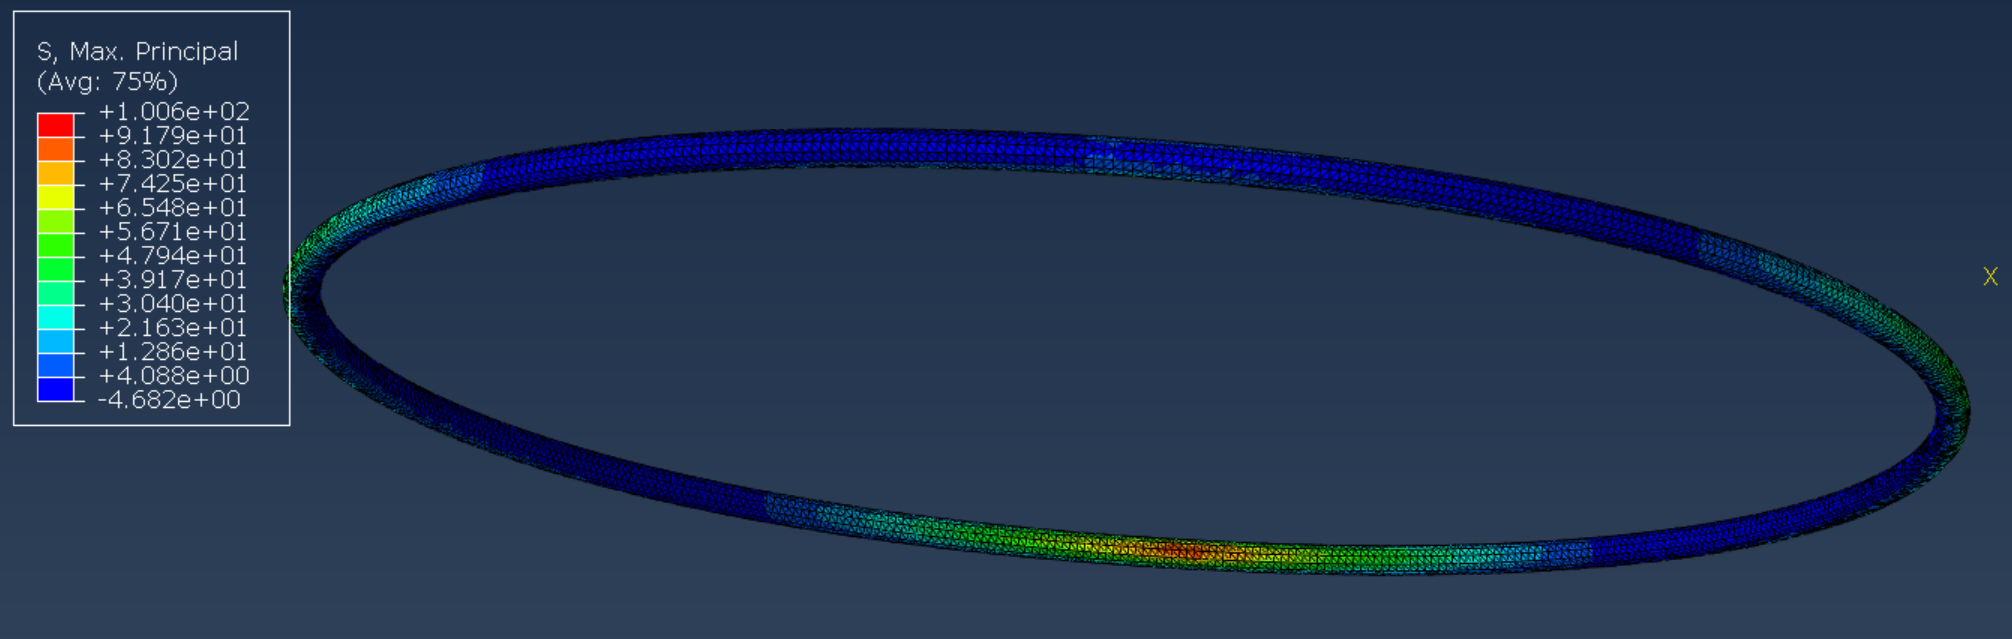
\includegraphics[width=400]{saut2/elf3.PNG}
\caption{Contraintes dans la roue lors de la compression par une force exercée à son sommet, obtenues par une analyse éléments finis linéaire. Les contraintes maximales se situent au niveau du rayon interne de la roue là où la force est exercée et dans la zone diamétralement opposée à cet endroit.}
\label{fig:elf2}
\end{figure}

Les paramètres des études éléments finis correspondent à une roue de rayon médian $R=0.9 m$, en nylon renforcé avec des fibres de carbone courtes à laquelle on applique la force de compression $F=F_2$.

\begin{figure}[h]
\def\svgwidth{240}
%% Creator: Inkscape inkscape 0.92.2, www.inkscape.org
%% PDF/EPS/PS + LaTeX output extension by Johan Engelen, 2010
%% Accompanies image file 'fle1.eps' (pdf, eps, ps)
%%
%% To include the image in your LaTeX document, write
%%   \input{<filename>.pdf_tex}
%%  instead of
%%   \includegraphics{<filename>.pdf}
%% To scale the image, write
%%   \def\svgwidth{<desired width>}
%%   \input{<filename>.pdf_tex}
%%  instead of
%%   \includegraphics[width=<desired width>]{<filename>.pdf}
%%
%% Images with a different path to the parent latex file can
%% be accessed with the `import' package (which may need to be
%% installed) using
%%   \usepackage{import}
%% in the preamble, and then including the image with
%%   \import{<path to file>}{<filename>.pdf_tex}
%% Alternatively, one can specify
%%   \graphicspath{{<path to file>/}}
%% 
%% For more information, please see info/svg-inkscape on CTAN:
%%   http://tug.ctan.org/tex-archive/info/svg-inkscape
%%
\begingroup%
  \makeatletter%
  \providecommand\color[2][]{%
    \errmessage{(Inkscape) Color is used for the text in Inkscape, but the package 'color.sty' is not loaded}%
    \renewcommand\color[2][]{}%
  }%
  \providecommand\transparent[1]{%
    \errmessage{(Inkscape) Transparency is used (non-zero) for the text in Inkscape, but the package 'transparent.sty' is not loaded}%
    \renewcommand\transparent[1]{}%
  }%
  \providecommand\rotatebox[2]{#2}%
  \ifx\svgwidth\undefined%
    \setlength{\unitlength}{344.79999138bp}%
    \ifx\svgscale\undefined%
      \relax%
    \else%
      \setlength{\unitlength}{\unitlength * \real{\svgscale}}%
    \fi%
  \else%
    \setlength{\unitlength}{\svgwidth}%
  \fi%
  \global\let\svgwidth\undefined%
  \global\let\svgscale\undefined%
  \makeatother%
  \begin{picture}(1,0.83526682)%
    \put(0,0){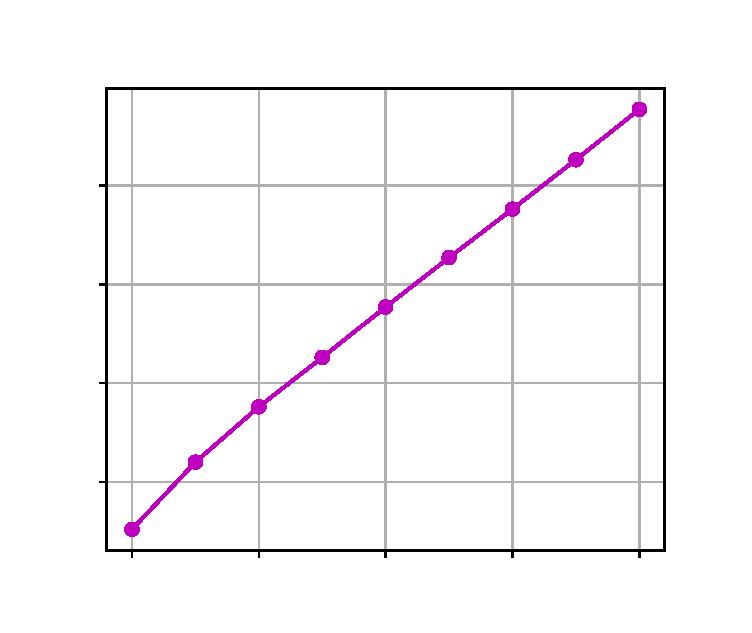
\includegraphics[width=\unitlength]{images_2ddl/fle1.eps}}%
    \put(0.14215545,0.044955423){\color[rgb]{0,0,0}\makebox(0,0)[lb]{\smash{10}}}%
    \put(0.3187007,0.044955423){\color[rgb]{0,0,0}\makebox(0,0)[lb]{\smash{20}}}%
    \put(0.49524652,0.044955423){\color[rgb]{0,0,0}\makebox(0,0)[lb]{\smash{30}}}%
    \put(0.67178944,0.044955423){\color[rgb]{0,0,0}\makebox(0,0)[lb]{\smash{40}}}%
    \put(0.84833527,0.044955423){\color[rgb]{0,0,0}\makebox(0,0)[lb]{\smash{50}}}%
    \put(0.056810122,0.17613689){\color[rgb]{0,0,0}\makebox(0,0)[lb]{\smash{10}}}%
    \put(0.056810122,0.3137094){\color[rgb]{0,0,0}\makebox(0,0)[lb]{\smash{20}}}%
    \put(0.056810122,0.4512848){\color[rgb]{0,0,0}\makebox(0,0)[lb]{\smash{30}}}%
    \put(0.056810122,0.58885731){\color[rgb]{0,0,0}\makebox(0,0)[lb]{\smash{40}}}%
    \put(0.025047303,0.31404872){\color[rgb]{0,0,0}\rotatebox{90}{\makebox(0,0)[lb]{\smash{$r_1 (mm)$}}}}%
    \put(0.45,0.0){\color[rgb]{0,0,0}\makebox(0,0)[lb]{\smash{$r_2 (mm)$}}}%
  \end{picture}%
\endgroup%

\def\svgwidth{240}
%% Creator: Inkscape inkscape 0.92.2, www.inkscape.org
%% PDF/EPS/PS + LaTeX output extension by Johan Engelen, 2010
%% Accompanies image file 'fle2.eps' (pdf, eps, ps)
%%
%% To include the image in your LaTeX document, write
%%   \input{<filename>.pdf_tex}
%%  instead of
%%   \includegraphics{<filename>.pdf}
%% To scale the image, write
%%   \def\svgwidth{<desired width>}
%%   \input{<filename>.pdf_tex}
%%  instead of
%%   \includegraphics[width=<desired width>]{<filename>.pdf}
%%
%% Images with a different path to the parent latex file can
%% be accessed with the `import' package (which may need to be
%% installed) using
%%   \usepackage{import}
%% in the preamble, and then including the image with
%%   \import{<path to file>}{<filename>.pdf_tex}
%% Alternatively, one can specify
%%   \graphicspath{{<path to file>/}}
%% 
%% For more information, please see info/svg-inkscape on CTAN:
%%   http://tug.ctan.org/tex-archive/info/svg-inkscape
%%
\begingroup%
  \makeatletter%
  \providecommand\color[2][]{%
    \errmessage{(Inkscape) Color is used for the text in Inkscape, but the package 'color.sty' is not loaded}%
    \renewcommand\color[2][]{}%
  }%
  \providecommand\transparent[1]{%
    \errmessage{(Inkscape) Transparency is used (non-zero) for the text in Inkscape, but the package 'transparent.sty' is not loaded}%
    \renewcommand\transparent[1]{}%
  }%
  \providecommand\rotatebox[2]{#2}%
  \ifx\svgwidth\undefined%
    \setlength{\unitlength}{344.79999138bp}%
    \ifx\svgscale\undefined%
      \relax%
    \else%
      \setlength{\unitlength}{\unitlength * \real{\svgscale}}%
    \fi%
  \else%
    \setlength{\unitlength}{\svgwidth}%
  \fi%
  \global\let\svgwidth\undefined%
  \global\let\svgscale\undefined%
  \makeatother%
  \begin{picture}(1,0.83526682)%
    \put(0,0){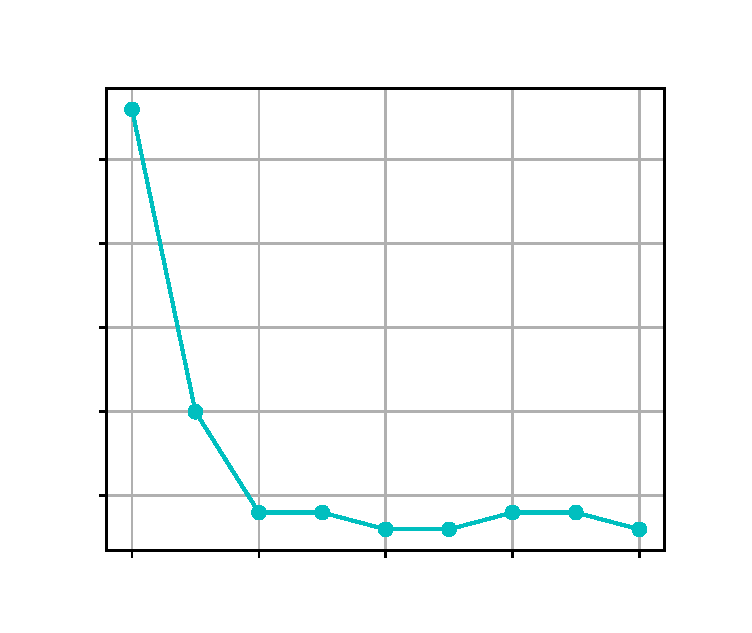
\includegraphics[width=\unitlength]{images_2ddl/fle2.eps}}%
    \put(0.14215545,0.044955423){\color[rgb]{0,0,0}\makebox(0,0)[lb]{\smash{10}}}%
    \put(0.3187007,0.044955423){\color[rgb]{0,0,0}\makebox(0,0)[lb]{\smash{20}}}%
    \put(0.49524652,0.044955423){\color[rgb]{0,0,0}\makebox(0,0)[lb]{\smash{30}}}%
    \put(0.67178944,0.044955423){\color[rgb]{0,0,0}\makebox(0,0)[lb]{\smash{40}}}%
    \put(0.84833527,0.044955423){\color[rgb]{0,0,0}\makebox(0,0)[lb]{\smash{50}}}%
    \put(0.045885673,0.15687645){\color[rgb]{0,0,0}\makebox(0,0)[lb]{\smash{2.5}}}%
    \put(0.045885673,0.27381352){\color[rgb]{0,0,0}\makebox(0,0)[lb]{\smash{3.0}}}%
    \put(0.045885673,0.39075116){\color[rgb]{0,0,0}\makebox(0,0)[lb]{\smash{3.5}}}%
    \put(0.045885673,0.50768852){\color[rgb]{0,0,0}\makebox(0,0)[lb]{\smash{4.0}}}%
    \put(0.045885673,0.62462587){\color[rgb]{0,0,0}\makebox(0,0)[lb]{\smash{4.5}}}%
    
    \put(0.49524652,0.0){\color[rgb]{0,0,0}\makebox(0,0)[lb]{\smash{$r_2 (mm)$}}}%
    \put(0.025,0.25896752){\color[rgb]{0,0,0}\rotatebox{90}{\makebox(0,0)[lb]{\smash{épaisseur $(mm)$}}}}%
  \end{picture}%
\endgroup%

\caption{Couples $(r_1,r_2)$ pour lesquels on à a la fois flambement et écoulement dans la roue en nylon renforcé aux fibres de carbone courtes, pour une force $F_2=4500 N$ appliquée à son sommet.}
\label{fig:fle12}
\end{figure}

\subsubsection{Limites en écoulement à l'impact}

Lorsque l'utilisateur saute avec la roue, la partie entre ses pieds et le sol est soumise à des contraintes dues à l'impact de l'atterrissage qui créent de l'écoulement et un écrasement de la section si son épaisseur n'est pas suffisante. 

Le saut peut s'effectuer pieds joints ou écartés. La configuration pieds joints étant celle qui génère le plus de contraintes, c'est la seule que nous étudierons.

De même que précédemment, pour chaque valeur du rayon externe $r_2$, compris entre $10 mm$ et $50 mm$, une étude linéaire par éléments finis nous donne le rayon interne $r_1$ à partir duquel il y a écoulement dans la section. \\
Pour cette étude, on modélise uniquement la partie inférieure de la roue, qu'on approxime par un cylindre auquel est appliqué la pression correspondant à la force $F_2$ répartie sur la surface de contact entre les pieds de l'utilisateur et la roue (figure \ref{fig:ecrasement}).

 \begin{figure}[h]
\centering
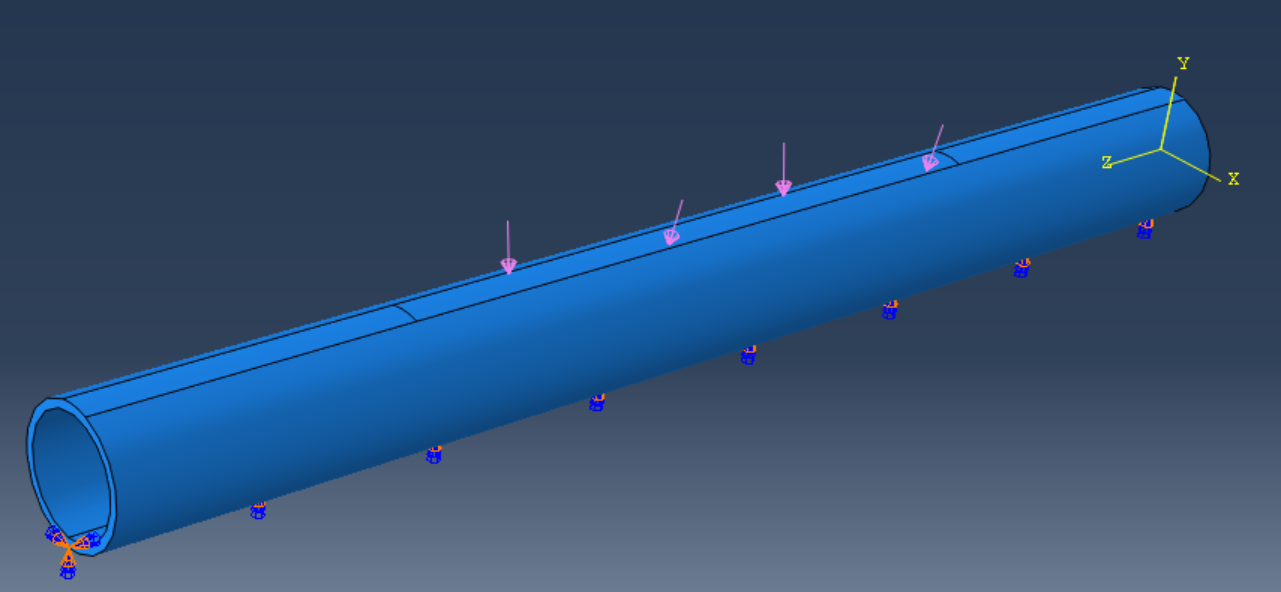
\includegraphics[width=290]{saut2/elf4.PNG}
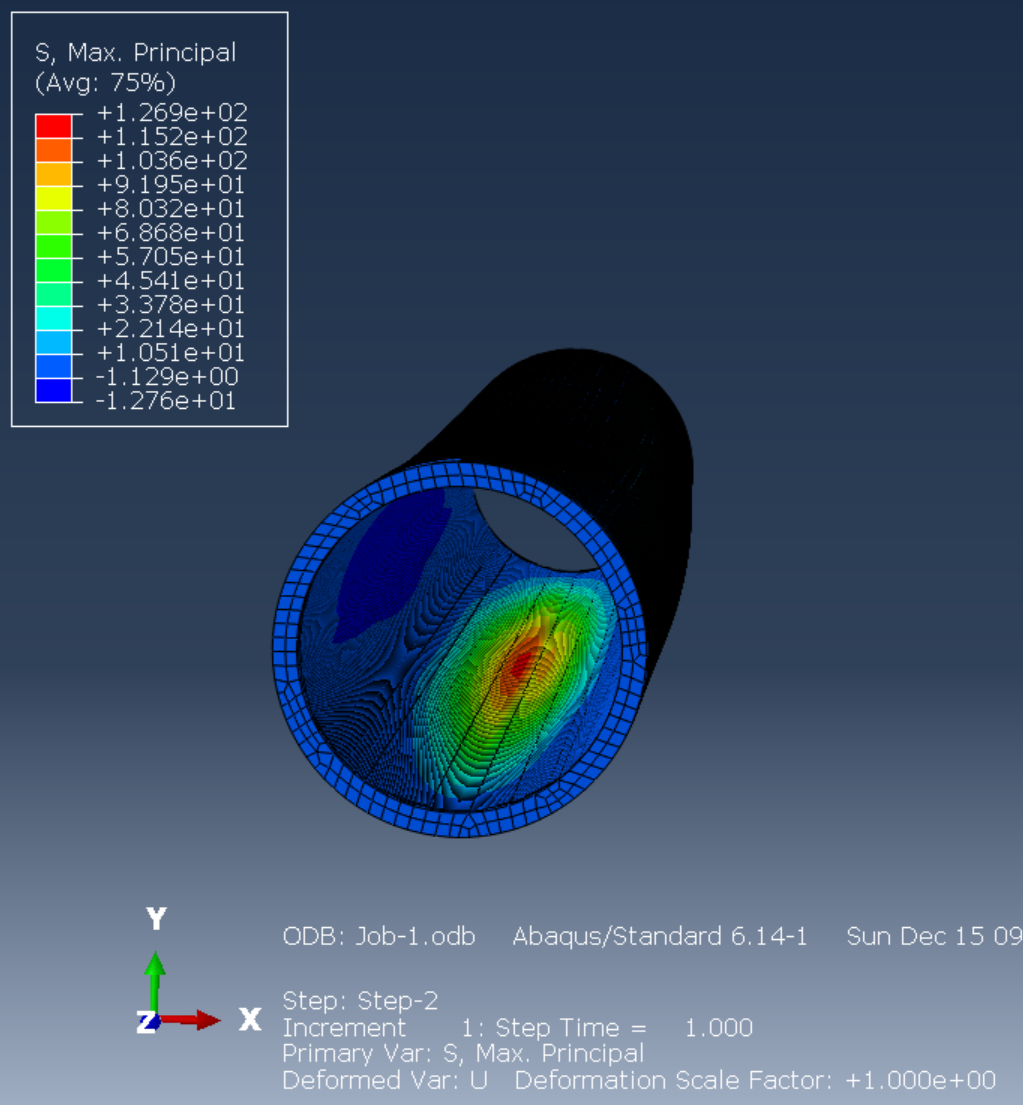
\includegraphics[width=170]{saut2/elf5.PNG}
\caption{Modélisation éléments finis de l'écrasement de la section de la roue entre les pieds de l'utilisateur et le sol lors de l'impact dû à l'atterrissage.}
\label{fig:ecrasement}
\end{figure}

\subsubsection{Limites en comportement linéaire}
Pour rester dans le domaine de comportement linéaire géométrique défini au début du chapitre la flèche $\delta$ imposée par l'utilisateur ne doit pas dépasser 10\% du rayon médian $R$. 
Cette condition s'applique au cas d'utilisation courant de la roue, le chargement correspondant est la force $F_1$.
On évalue la flèche avec son expression théorique: $\delta=F_1/k$, où $k$ est la constante élastique définie plus haut, pour une roue en nylon renforcé aux fibres de carbone courtes de rayon médian $R=0.9 m$. 
Pour chaque $r_2$ donné, on obtient ainsi la valeur maximale de $r_1$ pour rester dans le domaine linéaire (figure \ref{fig:fle4}). On remarque que pour $r_2=10 mm$ il n'est pas possible d'avoir un comportement linéaire, la courbe se trouvant entièrement au delà de la frontière. On éliminera donc le cas $r_2=10 mm$ pour la suite.

\begin{figure}
\centering
\def\svgwidth{350}
%% Creator: Inkscape inkscape 0.92.2, www.inkscape.org
%% PDF/EPS/PS + LaTeX output extension by Johan Engelen, 2010
%% Accompanies image file 'fle4.eps' (pdf, eps, ps)
%%
%% To include the image in your LaTeX document, write
%%   \input{<filename>.pdf_tex}
%%  instead of
%%   \includegraphics{<filename>.pdf}
%% To scale the image, write
%%   \def\svgwidth{<desired width>}
%%   \input{<filename>.pdf_tex}
%%  instead of
%%   \includegraphics[width=<desired width>]{<filename>.pdf}
%%
%% Images with a different path to the parent latex file can
%% be accessed with the `import' package (which may need to be
%% installed) using
%%   \usepackage{import}
%% in the preamble, and then including the image with
%%   \import{<path to file>}{<filename>.pdf_tex}
%% Alternatively, one can specify
%%   \graphicspath{{<path to file>/}}
%% 
%% For more information, please see info/svg-inkscape on CTAN:
%%   http://tug.ctan.org/tex-archive/info/svg-inkscape
%%
\begingroup%
  \makeatletter%
  \providecommand\color[2][]{%
    \errmessage{(Inkscape) Color is used for the text in Inkscape, but the package 'color.sty' is not loaded}%
    \renewcommand\color[2][]{}%
  }%
  \providecommand\transparent[1]{%
    \errmessage{(Inkscape) Transparency is used (non-zero) for the text in Inkscape, but the package 'transparent.sty' is not loaded}%
    \renewcommand\transparent[1]{}%
  }%
  \providecommand\rotatebox[2]{#2}%
  \ifx\svgwidth\undefined%
    \setlength{\unitlength}{632.22074835bp}%
    \ifx\svgscale\undefined%
      \relax%
    \else%
      \setlength{\unitlength}{\unitlength * \real{\svgscale}}%
    \fi%
  \else%
    \setlength{\unitlength}{\svgwidth}%
  \fi%
  \global\let\svgwidth\undefined%
  \global\let\svgscale\undefined%
  \makeatother%
  \begin{picture}(1,0.45553708)%
    \put(0,0){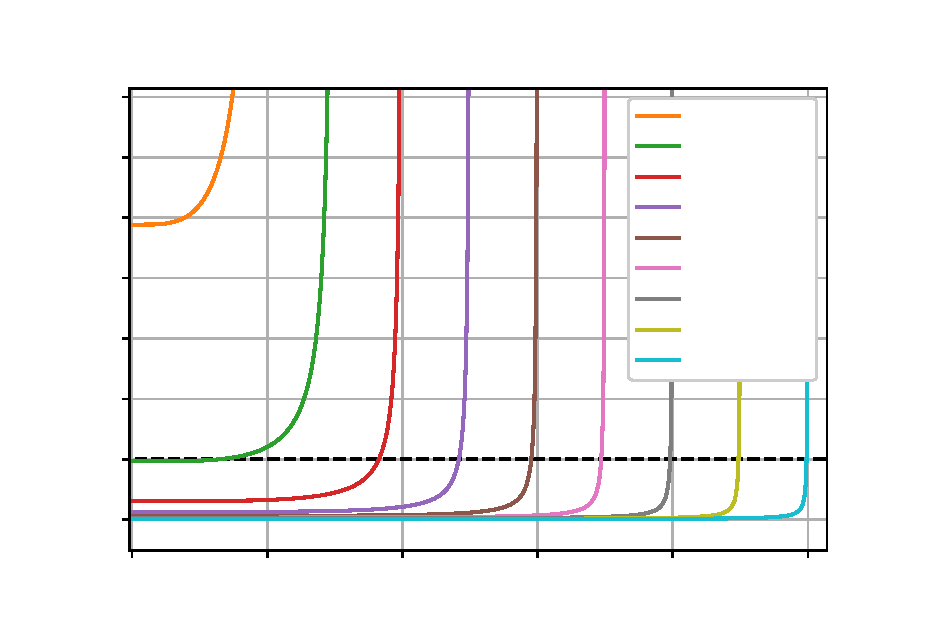
\includegraphics[width=\unitlength]{images_2ddl/fle4.eps}}%
    \put(0.12,0.02702584){\color[rgb]{0,0,0}\makebox(0,0)[lb]{\smash{0}}}%
    \put(0.26,0.02702584){\color[rgb]{0,0,0}\makebox(0,0)[lb]{\smash{10}}}%
    \put(0.41,0.02702584){\color[rgb]{0,0,0}\makebox(0,0)[lb]{\smash{20}}}%
    \put(0.56,0.02702584){\color[rgb]{0,0,0}\makebox(0,0)[lb]{\smash{30}}}%
    \put(0.71,0.02702584){\color[rgb]{0,0,0}\makebox(0,0)[lb]{\smash{40}}}%
    \put(0.86,0.02702584){\color[rgb]{0,0,0}\makebox(0,0)[lb]{\smash{50}}}%
    \put(0.06,0.1){\color[rgb]{0,0,0}\makebox(0,0)[lb]{\smash{0.0}}}%
    \put(0.06,0.165){\color[rgb]{0,0,0}\makebox(0,0)[lb]{\smash{0.1}}}%
    \put(0.06,0.23){\color[rgb]{0,0,0}\makebox(0,0)[lb]{\smash{0.2}}}%
    \put(0.06,0.3){\color[rgb]{0,0,0}\makebox(0,0)[lb]{\smash{0.3}}}%
    \put(0.06,0.365){\color[rgb]{0,0,0}\makebox(0,0)[lb]{\smash{0.4}}}%
    \put(0.06,0.435){\color[rgb]{0,0,0}\makebox(0,0)[lb]{\smash{0.5}}}%
    \put(0.06,0.5){\color[rgb]{0,0,0}\makebox(0,0)[lb]{\smash{0.6}}}%
    \put(0.06,0.565){\color[rgb]{0,0,0}\makebox(0,0)[lb]{\smash{0.7}}}%
    \put(0.03,0.3){\color[rgb]{0,0,0}\rotatebox{90}{\makebox(0,0)[lb]{\smash{$\delta / R$}}}}%
    \put(0.445,0.0){\color[rgb]{0,0,0}\makebox(0,0)[lb]{\smash{$r_1(mm)$}}}%
    \put(0.74,0.55){\color[rgb]{0,0,0}\makebox(0,0)[lb]{\smash{\footnotesize $r_2=10 mm$}}}%
    \put(0.74,0.515){\color[rgb]{0,0,0}\makebox(0,0)[lb]{\smash{\footnotesize $r_2=15 mm$}}}%
    \put(0.74,0.48){\color[rgb]{0,0,0}\makebox(0,0)[lb]{\smash{\footnotesize $r_2=20 mm$}}}%
    \put(0.74,0.445){\color[rgb]{0,0,0}\makebox(0,0)[lb]{\smash{\footnotesize $r_2=25 mm$}}}%
    \put(0.74,0.413){\color[rgb]{0,0,0}\makebox(0,0)[lb]{\smash{\footnotesize $r_2=30 mm$}}}%
    \put(0.74,0.38){\color[rgb]{0,0,0}\makebox(0,0)[lb]{\smash{\footnotesize $r_2=35 mm$}}}%
    \put(0.74,0.345){\color[rgb]{0,0,0}\makebox(0,0)[lb]{\smash{\footnotesize $r_2=40 mm$}}}%
    \put(0.74,0.31){\color[rgb]{0,0,0}\makebox(0,0)[lb]{\smash{\footnotesize $r_2=45 mm$}}}%
    \put(0.74,0.275){\color[rgb]{0,0,0}\makebox(0,0)[lb]{\smash{\footnotesize $r_2=50 mm$}}}%
  \end{picture}%
\endgroup%

\caption{Ratio $\delta/R$ en fonction de $r_1$ pour un $r_2$ donné. La droite horizontale en pointillés correspond à la valeur $0.1$ au delà de laquelle on quitte le domaine de comportement linéaire. L'intersection de cette droite avec chacune des courbes donne la valeur de $r_1$ à ne pas dépasser pour rester dans le domaine linéaire géométrique. Les calculs sont réalisés pour une roue en nylon renforcé aux fibres de carbone courtes de rayon médian $R=0.9 m$, avec une force $F_1=900N$ appliquée à son sommet.}
\label{fig:fle4}
\end{figure}

\subsubsection{Optimisation de la section pour le saut de la roue Cyr}
Les limites obtenues dans les trois sections précédentes sont combinées à l'étude de la hauteur maximale de saut en fonction de $r_1$, pour chaque $r_2$ compris entre $15 mm$ et $50 mm$ (figure \ref{fig:fle3}). On estime la hauteur de saut avec notre modèle à deux degrés de liberté en considérant que la roue est comprimée d'une force de $900N$ puis relâchée. Par exemple, pour $r_2=15 mm$ on obtient des sauts de plusieurs mètres lorsque $r_1$ avoisine les $14mm$, cependant on sortira de la zone de comportement linéaire, la roue sera sujette au flambement et à l'écoulement lors de sa compression et il y aura écrasement de section à l'impact lors des sauts. Pour chaque courbe, les points d'intersection avec chacune des trois limites de $r_1$ correspondent aux hauteurs de saut optimisées pour chaque type de limite.


\begin{figure}[h]
\centering
\def\svgwidth{500}
%% Creator: Inkscape inkscape 0.92.2, www.inkscape.org
%% PDF/EPS/PS + LaTeX output extension by Johan Engelen, 2010
%% Accompanies image file 'fle3.eps' (pdf, eps, ps)
%%
%% To include the image in your LaTeX document, write
%%   \input{<filename>.pdf_tex}
%%  instead of
%%   \includegraphics{<filename>.pdf}
%% To scale the image, write
%%   \def\svgwidth{<desired width>}
%%   \input{<filename>.pdf_tex}
%%  instead of
%%   \includegraphics[width=<desired width>]{<filename>.pdf}
%%
%% Images with a different path to the parent latex file can
%% be accessed with the `import' package (which may need to be
%% installed) using
%%   \usepackage{import}
%% in the preamble, and then including the image with
%%   \import{<path to file>}{<filename>.pdf_tex}
%% Alternatively, one can specify
%%   \graphicspath{{<path to file>/}}
%% 
%% For more information, please see info/svg-inkscape on CTAN:
%%   http://tug.ctan.org/tex-archive/info/svg-inkscape
%%
\begingroup%
  \makeatletter%
  \providecommand\color[2][]{%
    \errmessage{(Inkscape) Color is used for the text in Inkscape, but the package 'color.sty' is not loaded}%
    \renewcommand\color[2][]{}%
  }%
  \providecommand\transparent[1]{%
    \errmessage{(Inkscape) Transparency is used (non-zero) for the text in Inkscape, but the package 'transparent.sty' is not loaded}%
    \renewcommand\transparent[1]{}%
  }%
  \providecommand\rotatebox[2]{#2}%
  \ifx\svgwidth\undefined%
    \setlength{\unitlength}{575.9999856bp}%
    \ifx\svgscale\undefined%
      \relax%
    \else%
      \setlength{\unitlength}{\unitlength * \real{\svgscale}}%
    \fi%
  \else%
    \setlength{\unitlength}{\svgwidth}%
  \fi%
  \global\let\svgwidth\undefined%
  \global\let\svgscale\undefined%
  \makeatother%
  \begin{picture}(1,0.66111111)%
    \put(0,0){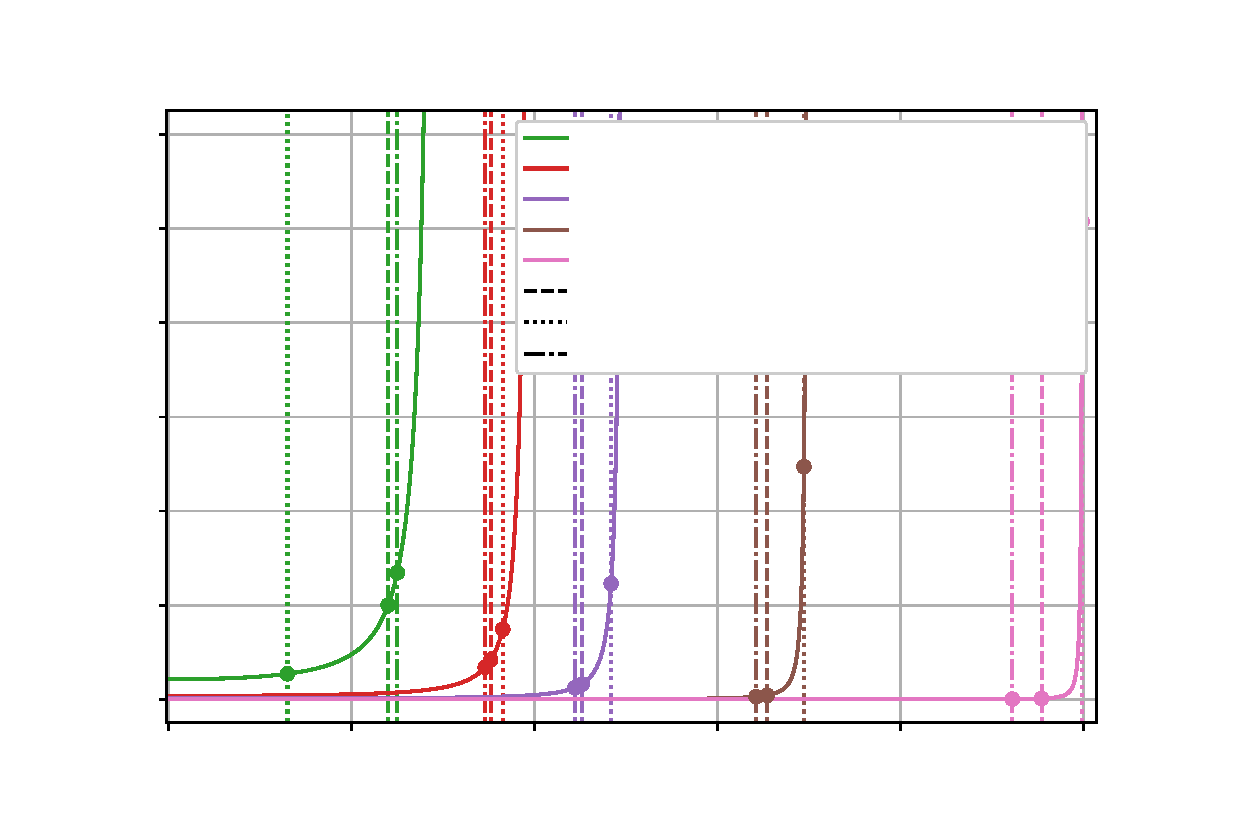
\includegraphics[width=\unitlength]{images_2ddl/fle3.eps}}%
    \put(0.12102726,0.04753889){\color[rgb]{0,0,0}\makebox(0,0)[lb]{\smash{0}}}%
    \put(0.26804688,0.04753889){\color[rgb]{0,0,0}\makebox(0,0)[lb]{\smash{10}}}%
    \put(0.42058854,0.04753889){\color[rgb]{0,0,0}\makebox(0,0)[lb]{\smash{20}}}%
    \put(0.57312847,0.04753889){\color[rgb]{0,0,0}\makebox(0,0)[lb]{\smash{30}}}%
    \put(0.7256684,0.04753889){\color[rgb]{0,0,0}\makebox(0,0)[lb]{\smash{40}}}%
    \put(0.87821007,0.04753889){\color[rgb]{0,0,0}\makebox(0,0)[lb]{\smash{50}}}%
    \put(0.1018066,0.08574358){\color[rgb]{0,0,0}\makebox(0,0)[lb]{\smash{0}}}%
    \put(0.1018066,0.16424358){\color[rgb]{0,0,0}\makebox(0,0)[lb]{\smash{2}}}%
    \put(0.1018066,0.24274306){\color[rgb]{0,0,0}\makebox(0,0)[lb]{\smash{4}}}%
    \put(0.1018066,0.32124306){\color[rgb]{0,0,0}\makebox(0,0)[lb]{\smash{6}}}%
    \put(0.1018066,0.39974306){\color[rgb]{0,0,0}\makebox(0,0)[lb]{\smash{8}}}%
    \put(0.09076615,0.47824306){\color[rgb]{0,0,0}\makebox(0,0)[lb]{\smash{10}}}%
    \put(0.09076615,0.55674132){\color[rgb]{0,0,0}\makebox(0,0)[lb]{\smash{12}}}%
    \put(0.07972552,0.28014063){\color[rgb]{0,0,0}\rotatebox{90}{\makebox(0,0)[lb]{\smash{$H_{max} (m)$}}}}%
    \put(0.47221181,0.55419097){\color[rgb]{0,0,0}\makebox(0,0)[lb]{\smash{$r_2=15 mm$}}}%
    \put(0.47221181,0.52872049){\color[rgb]{0,0,0}\makebox(0,0)[lb]{\smash{$r_2=20 mm$}}}%
    \put(0.47221181,0.50324826){\color[rgb]{0,0,0}\makebox(0,0)[lb]{\smash{$r_2=25 mm$}}}%
    \put(0.47221181,0.47777604){\color[rgb]{0,0,0}\makebox(0,0)[lb]{\smash{$r_2=35 mm$}}}%
    \put(0.47221181,0.45230382){\color[rgb]{0,0,0}\makebox(0,0)[lb]{\smash{$r_2=50 mm$}}}%
    \put(0.47221181,0.4268316){\color[rgb]{0,0,0}\makebox(0,0)[lb]{\smash{limite en flambement/écoulement}}}%
    \put(0.47221181,0.40065451){\color[rgb]{0,0,0}\makebox(0,0)[lb]{\smash{$\delta / R>0.1$}}}%
    \put(0.47221181,0.37447743){\color[rgb]{0,0,0}\makebox(0,0)[lb]{\smash{limite en écoulement saut pieds joints}}}%
    \put(0.475,0.02){\color[rgb]{0,0,0}\makebox(0,0)[lb]{\smash{$r_1(mm)$}}}%
  \end{picture}%
\endgroup%

\caption{Hauteur maximale de saut en fonction de $r_1$, pour des $r_2$ donnés. Les points d'intersection des courbes $H_{max}=f(r_1)$ avec les limites en pointillés correspondent aux valeurs pour lesquelles le saut de la roue est optimisé. Les calculs sont réalisés pour une roue en nylon renforcé aux fibres de carbone courtes de rayon médian $R=0.9 m$, avec la force $F_1$ appliquée à son sommet.}
\label{fig:fle3}
\end{figure}

Ces points d'intersections reliés donnent trois nouvelles courbes correspondant chacune à un type de limite: flambement-écoulement en compression, écoulement à l'impact, sortie du domaine géométrique linéaire (figure \ref{fig:fle51}). Pour chaque $r_2$, le point le plus à gauche donne la valeur optimale de $r_1$, permettant d'avoir une épaisseur de section aussi fine que possible et de maximiser $H_{max}$ sans dommages, en gardant un comportement linéaire.

\begin{figure}[h]
\centering
\def\svgwidth{450}
%% Creator: Inkscape inkscape 0.92.2, www.inkscape.org
%% PDF/EPS/PS + LaTeX output extension by Johan Engelen, 2010
%% Accompanies image file 'fle41.eps' (pdf, eps, ps)
%%
%% To include the image in your LaTeX document, write
%%   \input{<filename>.pdf_tex}
%%  instead of
%%   \includegraphics{<filename>.pdf}
%% To scale the image, write
%%   \def\svgwidth{<desired width>}
%%   \input{<filename>.pdf_tex}
%%  instead of
%%   \includegraphics[width=<desired width>]{<filename>.pdf}
%%
%% Images with a different path to the parent latex file can
%% be accessed with the `import' package (which may need to be
%% installed) using
%%   \usepackage{import}
%% in the preamble, and then including the image with
%%   \import{<path to file>}{<filename>.pdf_tex}
%% Alternatively, one can specify
%%   \graphicspath{{<path to file>/}}
%% 
%% For more information, please see info/svg-inkscape on CTAN:
%%   http://tug.ctan.org/tex-archive/info/svg-inkscape
%%
\begingroup%
  \makeatletter%
  \providecommand\color[2][]{%
    \errmessage{(Inkscape) Color is used for the text in Inkscape, but the package 'color.sty' is not loaded}%
    \renewcommand\color[2][]{}%
  }%
  \providecommand\transparent[1]{%
    \errmessage{(Inkscape) Transparency is used (non-zero) for the text in Inkscape, but the package 'transparent.sty' is not loaded}%
    \renewcommand\transparent[1]{}%
  }%
  \providecommand\rotatebox[2]{#2}%
  \ifx\svgwidth\undefined%
    \setlength{\unitlength}{602.31990694bp}%
    \ifx\svgscale\undefined%
      \relax%
    \else%
      \setlength{\unitlength}{\unitlength * \real{\svgscale}}%
    \fi%
  \else%
    \setlength{\unitlength}{\svgwidth}%
  \fi%
  \global\let\svgwidth\undefined%
  \global\let\svgscale\undefined%
  \makeatother%
  \begin{picture}(1,0.56554637)%
    \put(0,0){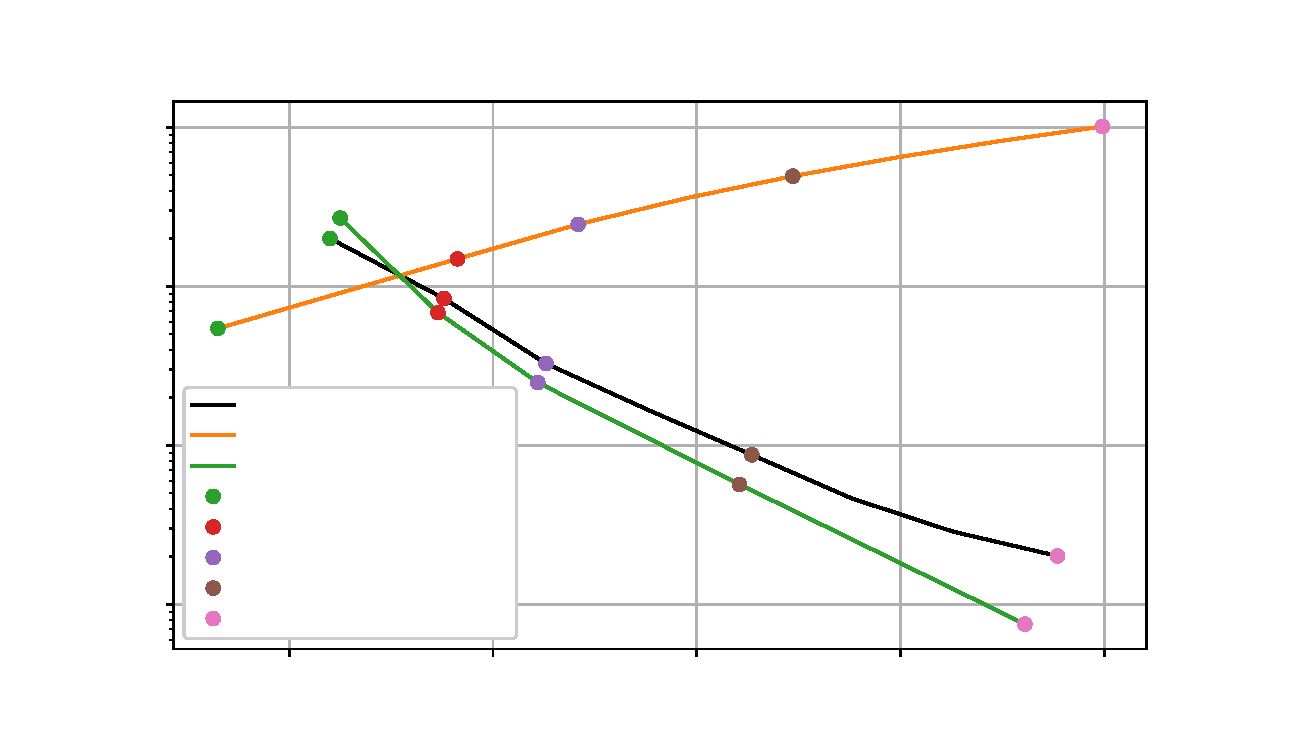
\includegraphics[width=\unitlength]{images_2ddl/fle41.eps}}%
    \put(0.20661598,0.03809743){\color[rgb]{0,0,0}\makebox(0,0)[lb]{\smash{10}}}%
    \put(0.36902801,0.03809743){\color[rgb]{0,0,0}\makebox(0,0)[lb]{\smash{20}}}%
    \put(0.53144004,0.03809743){\color[rgb]{0,0,0}\makebox(0,0)[lb]{\smash{30}}}%
    \put(0.69385207,0.03809743){\color[rgb]{0,0,0}\makebox(0,0)[lb]{\smash{40}}}%
    \put(0.85626575,0.03809743){\color[rgb]{0,0,0}\makebox(0,0)[lb]{\smash{50}}}%
    \put(0.067359896,0.09206078){\color[rgb]{0,0,0}\makebox(0,0)[lb]{\smash{$10^{-2}$}}}%
    \put(0.067359896,0.21808816){\color[rgb]{0,0,0}\makebox(0,0)[lb]{\smash{$10^{-1}$}}}%
    \put(0.078356045,0.34548557){\color[rgb]{0,0,0}\makebox(0,0)[lb]{\smash{$10^0$}}}%
    \put(0.078356045,0.47151162){\color[rgb]{0,0,0}\makebox(0,0)[lb]{\smash{$10^1$}}}%
    \put(0.06304079,0.23476368){\color[rgb]{0,0,0}\rotatebox{90}{\makebox(0,0)[lb]{\smash{$H_{ma x}(m)$}}}}%
    \put(0.5,0.01){\color[rgb]{0,0,0}\makebox(0,0)[lb]{\smash{$r_1 (mm)$}}}%
    \put(0.188649545,0.25123168){\color[rgb]{0,0,0}\makebox(0,0)[lb]{\smash{\scriptsize flambement/écoulement}}}%
    \put(0.18649545,0.22687253){\color[rgb]{0,0,0}\makebox(0,0)[lb]{\smash{\footnotesize $\delta/R>0.1$}}}%
    \put(0.18649545,0.20251338){\color[rgb]{0,0,0}\makebox(0,0)[lb]{\smash{\scriptsize écrasement de section}}}%
    \put(0.18649545,0.17815423){\color[rgb]{0,0,0}\makebox(0,0)[lb]{\smash{\footnotesize $r_2=15 mm$}}}%
    \put(0.18649545,0.15379592){\color[rgb]{0,0,0}\makebox(0,0)[lb]{\smash{\footnotesize $r_2=20 mm$}}}%
    \put(0.18649545,0.1294371){\color[rgb]{0,0,0}\makebox(0,0)[lb]{\smash{\footnotesize $r_2=25 mm$}}}%
    \put(0.18649545,0.10507812){\color[rgb]{0,0,0}\makebox(0,0)[lb]{\smash{\footnotesize $r_2=35 mm$}}}%
    \put(0.18649545,0.08071914){\color[rgb]{0,0,0}\makebox(0,0)[lb]{\smash{\footnotesize $r_2=50 mm$}}}%
  \end{picture}%
\endgroup%

\caption{Hauteur maximale de saut aux points d'optimisation $(r_1,r_2)$. Les calculs sont réalisés pour une roue en nylon renforcé aux fibres de carbone courtes de rayon médian $R=0.9 m$, avec la force $F_1$ appliquée à son sommet.}
\label{fig:fle51}
\end{figure}

D'après la figure \ref{fig:fle51}, la section optimale correspond à un $r_2$ compris entre $15mm$ et $20mm$. On raffine donc cette zone de l'étude (figure \ref{fig:fle52}).

\begin{figure}[h]
\centering
\def\svgwidth{400}
%% Creator: Inkscape inkscape 0.92.2, www.inkscape.org
%% PDF/EPS/PS + LaTeX output extension by Johan Engelen, 2010
%% Accompanies image file 'fle6.eps' (pdf, eps, ps)
%%
%% To include the image in your LaTeX document, write
%%   \input{<filename>.pdf_tex}
%%  instead of
%%   \includegraphics{<filename>.pdf}
%% To scale the image, write
%%   \def\svgwidth{<desired width>}
%%   \input{<filename>.pdf_tex}
%%  instead of
%%   \includegraphics[width=<desired width>]{<filename>.pdf}
%%
%% Images with a different path to the parent latex file can
%% be accessed with the `import' package (which may need to be
%% installed) using
%%   \usepackage{import}
%% in the preamble, and then including the image with
%%   \import{<path to file>}{<filename>.pdf_tex}
%% Alternatively, one can specify
%%   \graphicspath{{<path to file>/}}
%% 
%% For more information, please see info/svg-inkscape on CTAN:
%%   http://tug.ctan.org/tex-archive/info/svg-inkscape
%%
\begingroup%
  \makeatletter%
  \providecommand\color[2][]{%
    \errmessage{(Inkscape) Color is used for the text in Inkscape, but the package 'color.sty' is not loaded}%
    \renewcommand\color[2][]{}%
  }%
  \providecommand\transparent[1]{%
    \errmessage{(Inkscape) Transparency is used (non-zero) for the text in Inkscape, but the package 'transparent.sty' is not loaded}%
    \renewcommand\transparent[1]{}%
  }%
  \providecommand\rotatebox[2]{#2}%
  \ifx\svgwidth\undefined%
    \setlength{\unitlength}{480.11991bp}%
    \ifx\svgscale\undefined%
      \relax%
    \else%
      \setlength{\unitlength}{\unitlength * \real{\svgscale}}%
    \fi%
  \else%
    \setlength{\unitlength}{\svgwidth}%
  \fi%
  \global\let\svgwidth\undefined%
  \global\let\svgscale\undefined%
  \makeatother%
  \begin{picture}(1,0.73473343)%
    \put(0,0){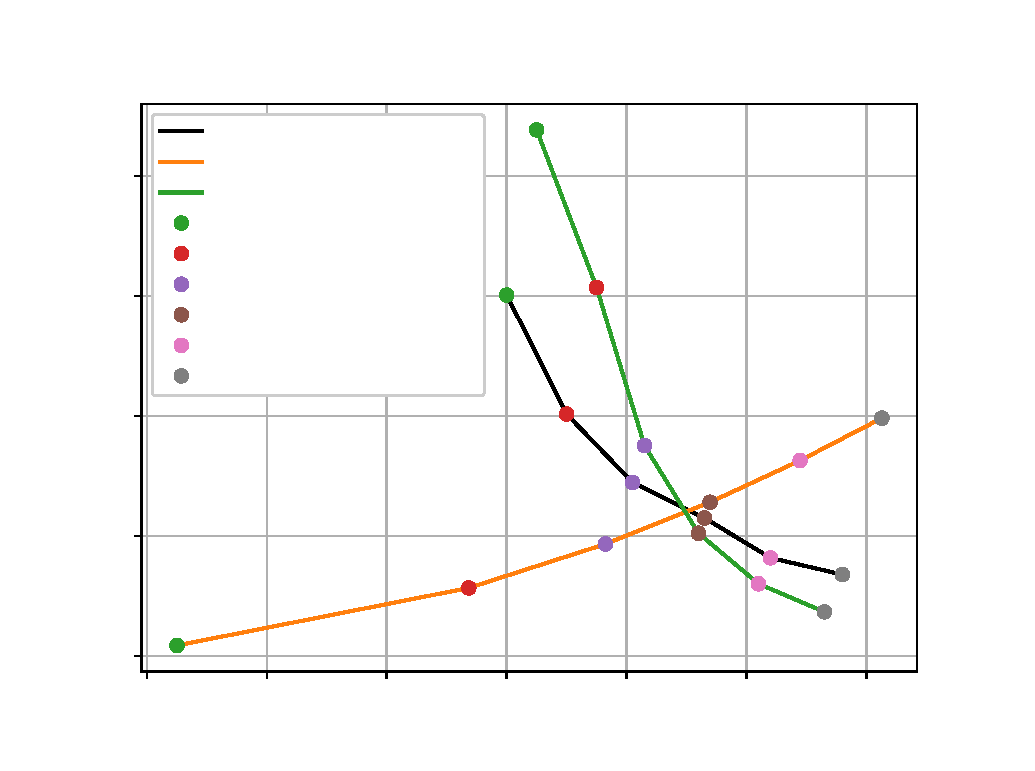
\includegraphics[width=\unitlength]{images_2ddl/fle6.eps}}%
    \put(0.12374434,0.05059935){\color[rgb]{0,0,0}\makebox(0,0)[lb]{\smash{6}}}%
    \put(0.24359106,0.05059935){\color[rgb]{0,0,0}\makebox(0,0)[lb]{\smash{8}}}%
    \put(0.35681486,0.05059935){\color[rgb]{0,0,0}\makebox(0,0)[lb]{\smash{10}}}%
    \put(0.47665992,0.05059935){\color[rgb]{0,0,0}\makebox(0,0)[lb]{\smash{12}}}%
    \put(0.59650706,0.05059935){\color[rgb]{0,0,0}\makebox(0,0)[lb]{\smash{14}}}%
    \put(0.7163542,0.05059935){\color[rgb]{0,0,0}\makebox(0,0)[lb]{\smash{16}}}%
    \put(0.83620134,0.05059935){\color[rgb]{0,0,0}\makebox(0,0)[lb]{\smash{18}}}%
    \put(0.07732198,0.08822412){\color[rgb]{0,0,0}\makebox(0,0)[lb]{\smash{0.5}}}%
    \put(0.07732198,0.20819831){\color[rgb]{0,0,0}\makebox(0,0)[lb]{\smash{1.0}}}%
    \put(0.07732198,0.3281725){\color[rgb]{0,0,0}\makebox(0,0)[lb]{\smash{1.5}}}%
    \put(0.07732198,0.44814878){\color[rgb]{0,0,0}\makebox(0,0)[lb]{\smash{2.0}}}%
    \put(0.07732198,0.56812297){\color[rgb]{0,0,0}\makebox(0,0)[lb]{\smash{2.5}}}%
    \put(0.06407654,0.30713401){\color[rgb]{0,0,0}\rotatebox{90}{\makebox(0,0)[lb]{\smash{$H_{max} (m)$}}}}%
    \put(0.45665992,0.02){\color[rgb]{0,0,0}\makebox(0,0)[lb]{\smash{$r_1 (mm)$}}}%
    \put(0.2020956,0.61339708){\color[rgb]{0,0,0}\makebox(0,0)[lb]{\smash{\footnotesize flambement/écoulement}}}%
    \put(0.2020956,0.58283804){\color[rgb]{0,0,0}\makebox(0,0)[lb]{\smash{\small $\delta/R>0.1$}}}%
    \put(0.2020956,0.55227901){\color[rgb]{0,0,0}\makebox(0,0)[lb]{\smash{\footnotesize écrasement de section}}}%
    \put(0.2020956,0.52171998){\color[rgb]{0,0,0}\makebox(0,0)[lb]{\smash{$r_2=15 mm$}}}%
    \put(0.2020956,0.49116095){\color[rgb]{0,0,0}\makebox(0,0)[lb]{\smash{$r_2=16 mm$}}}%
    \put(0.2020956,0.46060192){\color[rgb]{0,0,0}\makebox(0,0)[lb]{\smash{$r_2=17 mm$}}}%
    \put(0.2020956,0.43004497){\color[rgb]{0,0,0}\makebox(0,0)[lb]{\smash{$r_2=18 mm$}}}%
    \put(0.2020956,0.39948594){\color[rgb]{0,0,0}\makebox(0,0)[lb]{\smash{$r_2=19 mm$}}}%
    \put(0.2020956,0.3689269){\color[rgb]{0,0,0}\makebox(0,0)[lb]{\smash{$r_2=20 mm$}}}%
  \end{picture}%
\endgroup%

\caption{Étude raffinée}
\label{fig:fle52}
\end{figure}
Pour chaque $r_2$ compris entre $15mm$ et $50mm$, on garde la plus basse des trois limites de $r_1$ (figure \ref{fig:fle5}). La courbe obtenue donne la valeur de $H_{max}$ aux points d'optimisation $(r_1,r_2)$ qui permettent de la maximiser tout en respectant chaque limite. 
Les dimensions de section optimales sont ainsi $r_2=18 mm$ et $r_1=15.2 mm$, et la hauteur maximale de saut correspondante est $H_{max}=1.01 m$.
\begin{figure}[h]
\centering
\def\svgwidth{300}
%% Creator: Inkscape inkscape 0.92.2, www.inkscape.org
%% PDF/EPS/PS + LaTeX output extension by Johan Engelen, 2010
%% Accompanies image file 'fle7.eps' (pdf, eps, ps)
%%
%% To include the image in your LaTeX document, write
%%   \input{<filename>.pdf_tex}
%%  instead of
%%   \includegraphics{<filename>.pdf}
%% To scale the image, write
%%   \def\svgwidth{<desired width>}
%%   \input{<filename>.pdf_tex}
%%  instead of
%%   \includegraphics[width=<desired width>]{<filename>.pdf}
%%
%% Images with a different path to the parent latex file can
%% be accessed with the `import' package (which may need to be
%% installed) using
%%   \usepackage{import}
%% in the preamble, and then including the image with
%%   \import{<path to file>}{<filename>.pdf_tex}
%% Alternatively, one can specify
%%   \graphicspath{{<path to file>/}}
%% 
%% For more information, please see info/svg-inkscape on CTAN:
%%   http://tug.ctan.org/tex-archive/info/svg-inkscape
%%
\begingroup%
  \makeatletter%
  \providecommand\color[2][]{%
    \errmessage{(Inkscape) Color is used for the text in Inkscape, but the package 'color.sty' is not loaded}%
    \renewcommand\color[2][]{}%
  }%
  \providecommand\transparent[1]{%
    \errmessage{(Inkscape) Transparency is used (non-zero) for the text in Inkscape, but the package 'transparent.sty' is not loaded}%
    \renewcommand\transparent[1]{}%
  }%
  \providecommand\rotatebox[2]{#2}%
  \ifx\svgwidth\undefined%
    \setlength{\unitlength}{344.79999138bp}%
    \ifx\svgscale\undefined%
      \relax%
    \else%
      \setlength{\unitlength}{\unitlength * \real{\svgscale}}%
    \fi%
  \else%
    \setlength{\unitlength}{\svgwidth}%
  \fi%
  \global\let\svgwidth\undefined%
  \global\let\svgscale\undefined%
  \makeatother%
  \begin{picture}(1,0.83526682)%
    \put(0,0){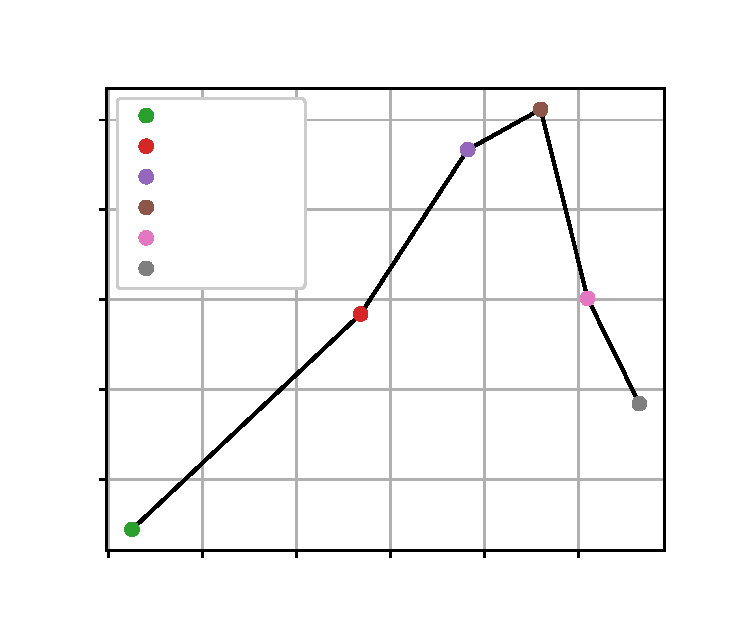
\includegraphics[width=\unitlength]{images_2ddl/fle7.eps}}%
    \put(0.11875435,0.04955423){\color[rgb]{0,0,0}\makebox(0,0)[lb]{\smash{6}}}%
    \put(0.24951508,0.04955423){\color[rgb]{0,0,0}\makebox(0,0)[lb]{\smash{8}}}%
    \put(0.37105568,0.04955423){\color[rgb]{0,0,0}\makebox(0,0)[lb]{\smash{10}}}%
    \put(0.50181845,0.04955423){\color[rgb]{0,0,0}\makebox(0,0)[lb]{\smash{12}}}%
    \put(0.63257831,0.04955423){\color[rgb]{0,0,0}\makebox(0,0)[lb]{\smash{14}}}%
    \put(0.76334107,0.04955423){\color[rgb]{0,0,0}\makebox(0,0)[lb]{\smash{16}}}%
    \put(0.05885673,0.17975667){\color[rgb]{0,0,0}\makebox(0,0)[lb]{\smash{0.6}}}%
    \put(0.05885673,0.30485209){\color[rgb]{0,0,0}\makebox(0,0)[lb]{\smash{0.7}}}%
    \put(0.05885673,0.4299449){\color[rgb]{0,0,0}\makebox(0,0)[lb]{\smash{0.8}}}%
    \put(0.05885673,0.5550377){\color[rgb]{0,0,0}\makebox(0,0)[lb]{\smash{0.9}}}%
    \put(0.05885673,0.68013051){\color[rgb]{0,0,0}\makebox(0,0)[lb]{\smash{1.0}}}%
    \put(0.04041299,0.33361079){\color[rgb]{0,0,0}\rotatebox{90}{\makebox(0,0)[lb]{\smash{$H_{max} (m)$}}}}%
    \put(0.470181845,0.01){\color[rgb]{0,0,0}\makebox(0,0)[lb]{\smash{$r_1 (mm)$}}}%
    \put(0.2,0.68690835){\color[rgb]{0,0,0}\makebox(0,0)[lb]{\smash{$r_2=15 mm$}}}%
    \put(0.2,0.64435615){\color[rgb]{0,0,0}\makebox(0,0)[lb]{\smash{$r_2=16 mm$}}}%
    \put(0.2,0.60180394){\color[rgb]{0,0,0}\makebox(0,0)[lb]{\smash{$r_2=17 mm$}}}%
    \put(0.2,0.55925174){\color[rgb]{0,0,0}\makebox(0,0)[lb]{\smash{$r_2=18 mm$}}}%
    \put(0.2,0.51670244){\color[rgb]{0,0,0}\makebox(0,0)[lb]{\smash{$r_2=19 mm$}}}%
    \put(0.2,0.47415023){\color[rgb]{0,0,0}\makebox(0,0)[lb]{\smash{$r_2=20 mm$}}}%
  \end{picture}%
\endgroup%

\caption{Hauteur maximale de saut aux points d'optimisation $(r_1,r_2)$. Les calculs sont réalisés pour une roue en nylon renforcé aux fibres de carbone courtes de rayon médian $R=0.9 m$, avec la force $F_1$ appliquée à son sommet.}
\label{fig:fle5}
\end{figure}


\subsection{Comparaison avec les points de l'article \textit{Jumping hoops}}
Dans leur article \textit{Jumping hoops} \cite{yangkim}, présenté au chapitre \ref{sec:RevLitt}, Yang et Kim étudient le saut d'anneaux comprimés puis relâchés.
Leur modèle théorique est basé sur des bilans énergétiques réalisés au moment où l'anneau quitte le sol et au moment où son centre de gravité atteint sa hauteur maximale, puis complété par leurs résultats expérimentaux (figure \ref{fig:ykres}).

\begin{figure}[htb]
\centering
\includegraphics[width=4.5in]{images_2ddl/ykres.png}
\caption{Résultats expérimentaux de Yang et Kim, sous forme de graphique adimensionnel. $H_{max}$ représente la hauteur maximale du saut, $h_c=\frac{E}{\rho g}$, où $E$ est le module d'Young, $\rho$ la masse volumique et $g$ l'accélération gravitationnelle. $\tau$ représente la longueur d'une des côtés de la section (l'autre, $w$ est fixé à 3 mm), $R$ est le rayon médian de la roue et $\delta$ est la flèche initiale imposée.}
\label{fig:ykres}
\end{figure}


On superpose les résultats expérimentaux de Yang et Kim et les courbes issues de nos modèles théoriques (figures \ref{fig:ykmae} et \ref{fig:yke}).
Pour $H_{max}$, les résultats expérimentaux de Yang et Kim concordent avec notre modèle théorique à deux degrés de liberté.
Pour le ratio d'efficacité énergétique $\dfrac{E_{p.g}}{E_{tot}}$, on observe des différences entre notre modèle théorique et les résultats expérimentaux de Yang et Kim.
Ces différences s'expliquent par la dissipation d'énergie due à la force de traînée que nous avons choisi de négliger dans notre modèle, et par un comportement non linéaire du coefficient de raideur $k$. Pour vérifier cette dernière supposition, nous calculons la valeur du ratio $\dfrac{\delta}{R}$ et la comparer à la valeur limite $0.1$ que nous avions définie au début du chapitre, au delà de laquelle on sort de la zone de comportement linéaire.

\begin{figure}[htb]
\centering
\def\svgwidth{320}
%% Creator: Inkscape inkscape 0.92.2, www.inkscape.org
%% PDF/EPS/PS + LaTeX output extension by Johan Engelen, 2010
%% Accompanies image file 'ykmae1.eps' (pdf, eps, ps)
%%
%% To include the image in your LaTeX document, write
%%   \input{<filename>.pdf_tex}
%%  instead of
%%   \includegraphics{<filename>.pdf}
%% To scale the image, write
%%   \def\svgwidth{<desired width>}
%%   \input{<filename>.pdf_tex}
%%  instead of
%%   \includegraphics[width=<desired width>]{<filename>.pdf}
%%
%% Images with a different path to the parent latex file can
%% be accessed with the `import' package (which may need to be
%% installed) using
%%   \usepackage{import}
%% in the preamble, and then including the image with
%%   \import{<path to file>}{<filename>.pdf_tex}
%% Alternatively, one can specify
%%   \graphicspath{{<path to file>/}}
%% 
%% For more information, please see info/svg-inkscape on CTAN:
%%   http://tug.ctan.org/tex-archive/info/svg-inkscape
%%
\begingroup%
  \makeatletter%
  \providecommand\color[2][]{%
    \errmessage{(Inkscape) Color is used for the text in Inkscape, but the package 'color.sty' is not loaded}%
    \renewcommand\color[2][]{}%
  }%
  \providecommand\transparent[1]{%
    \errmessage{(Inkscape) Transparency is used (non-zero) for the text in Inkscape, but the package 'transparent.sty' is not loaded}%
    \renewcommand\transparent[1]{}%
  }%
  \providecommand\rotatebox[2]{#2}%
  \ifx\svgwidth\undefined%
    \setlength{\unitlength}{395.9999901bp}%
    \ifx\svgscale\undefined%
      \relax%
    \else%
      \setlength{\unitlength}{\unitlength * \real{\svgscale}}%
    \fi%
  \else%
    \setlength{\unitlength}{\svgwidth}%
  \fi%
  \global\let\svgwidth\undefined%
  \global\let\svgscale\undefined%
  \makeatother%
  \begin{picture}(1,0.833939)%
    \put(0,0){\includegraphics[width=\unitlength]{images_2ddl/ykmae1.eps}}%
    \put(0.14153535,0.05494683){\color[rgb]{0,0,0}\makebox(0,0)[lb]{\smash{0}}}%
    \put(0.26236869,0.05494683){\color[rgb]{0,0,0}\makebox(0,0)[lb]{\smash{500}}}%
    \put(0.39123232,0.05494683){\color[rgb]{0,0,0}\makebox(0,0)[lb]{\smash{1000}}}%
    \put(0.52812626,0.05494683){\color[rgb]{0,0,0}\makebox(0,0)[lb]{\smash{1500}}}%
    \put(0.6650202,0.05494683){\color[rgb]{0,0,0}\makebox(0,0)[lb]{\smash{2000}}}%
    \put(0.80191162,0.05494683){\color[rgb]{0,0,0}\makebox(0,0)[lb]{\smash{2500}}}%
    \put(0.06,0.09675819){\color[rgb]{0,0,0}\makebox(0,0)[lb]{\smash{0.0}}}%
    \put(0.06,0.23034304){\color[rgb]{0,0,0}\makebox(0,0)[lb]{\smash{5.0}}}%
    \put(0.045109697,0.365){\color[rgb]{0,0,0}\makebox(0,0)[lb]{\smash{10.0}}}%
    \put(0.045109697,0.505){\color[rgb]{0,0,0}\makebox(0,0)[lb]{\smash{15.0}}}%
    \put(0.045109697,0.645){\color[rgb]{0,0,0}\makebox(0,0)[lb]{\smash{20.0}}}%
    \put(0.025,0.33304759){\color[rgb]{0,0,0}\rotatebox{90}{\makebox(0,0)[lb]{\smash{$H_{max}/R$}}}}%
    \put(0.21843434,0.6914693){\color[rgb]{0,0,0}\makebox(0,0)[lb]{\smash{\small modèle théorique 2DDL}}}%
    \put(0.21843434,0.65442132){\color[rgb]{0,0,0}\makebox(0,0)[lb]{\smash{\small Y\&K acier (120,30)}}}%
    \put(0.21843434,0.61737082){\color[rgb]{0,0,0}\makebox(0,0)[lb]{\smash{\small Y\&K polyimide (125,10)}}}%
    \put(0.21843434,0.58032031){\color[rgb]{0,0,0}\makebox(0,0)[lb]{\smash{\small Y\&K polyimide (125,15)}}}%
    \put(0.21843434,0.54326981){\color[rgb]{0,0,0}\makebox(0,0)[lb]{\smash{\small Y\&K polyimide (125,20)}}}%
    \put(0.21843434,0.5062193){\color[rgb]{0,0,0}\makebox(0,0)[lb]{\smash{\small Y\&K polyimide (75,10)}}}%
    \put(0.21843434,0.4691688){\color[rgb]{0,0,0}\makebox(0,0)[lb]{\smash{\small Y\&K polyimide (75,15)}}}%
    \put(0.21843434,0.43211829){\color[rgb]{0,0,0}\makebox(0,0)[lb]{\smash{\small Y\&K polyimide (75,25)}}}%
    \put(0.4,0.01){\color[rgb]{0,0,0}\makebox(0,0)[lb]{\smash{ $F^2 R/(E \rho g I A)$}}}%
  \end{picture}%
\endgroup%

\caption{Graphique adimensionnel des variations de $H_{max}$ en fonction des paramètres déterminants du modèle}
\label{fig:ykmae}
\end{figure}

\begin{figure}[htb]
\centering
\def\svgwidth{320}
%% Creator: Inkscape inkscape 0.92.2, www.inkscape.org
%% PDF/EPS/PS + LaTeX output extension by Johan Engelen, 2010
%% Accompanies image file 'yke3.eps' (pdf, eps, ps)
%%
%% To include the image in your LaTeX document, write
%%   \input{<filename>.pdf_tex}
%%  instead of
%%   \includegraphics{<filename>.pdf}
%% To scale the image, write
%%   \def\svgwidth{<desired width>}
%%   \input{<filename>.pdf_tex}
%%  instead of
%%   \includegraphics[width=<desired width>]{<filename>.pdf}
%%
%% Images with a different path to the parent latex file can
%% be accessed with the `import' package (which may need to be
%% installed) using
%%   \usepackage{import}
%% in the preamble, and then including the image with
%%   \import{<path to file>}{<filename>.pdf_tex}
%% Alternatively, one can specify
%%   \graphicspath{{<path to file>/}}
%% 
%% For more information, please see info/svg-inkscape on CTAN:
%%   http://tug.ctan.org/tex-archive/info/svg-inkscape
%%
\begingroup%
  \makeatletter%
  \providecommand\color[2][]{%
    \errmessage{(Inkscape) Color is used for the text in Inkscape, but the package 'color.sty' is not loaded}%
    \renewcommand\color[2][]{}%
  }%
  \providecommand\transparent[1]{%
    \errmessage{(Inkscape) Transparency is used (non-zero) for the text in Inkscape, but the package 'transparent.sty' is not loaded}%
    \renewcommand\transparent[1]{}%
  }%
  \providecommand\rotatebox[2]{#2}%
  \ifx\svgwidth\undefined%
    \setlength{\unitlength}{690.59998274bp}%
    \ifx\svgscale\undefined%
      \relax%
    \else%
      \setlength{\unitlength}{\unitlength * \real{\svgscale}}%
    \fi%
  \else%
    \setlength{\unitlength}{\svgwidth}%
  \fi%
  \global\let\svgwidth\undefined%
  \global\let\svgscale\undefined%
  \makeatother%
  \begin{picture}(1,0.83405734)%
    \put(0,0){\includegraphics[width=\unitlength]{images_2ddl/yke3.eps}}%
    \put(0.11819679,0.055061454){\color[rgb]{0,0,0}\makebox(0,0)[lb]{\smash{0}}}%
    \put(0.20939183,0.055061454){\color[rgb]{0,0,0}\makebox(0,0)[lb]{\smash{20}}}%
    \put(0.30919056,0.055061454){\color[rgb]{0,0,0}\makebox(0,0)[lb]{\smash{40}}}%
    \put(0.40898928,0.055061454){\color[rgb]{0,0,0}\makebox(0,0)[lb]{\smash{60}}}%
    \put(0.50878801,0.055061454){\color[rgb]{0,0,0}\makebox(0,0)[lb]{\smash{80}}}%
    \put(0.60398349,0.055061454){\color[rgb]{0,0,0}\makebox(0,0)[lb]{\smash{100}}}%
    \put(0.70378222,0.055061454){\color[rgb]{0,0,0}\makebox(0,0)[lb]{\smash{120}}}%
    \put(0.80358094,0.055061454){\color[rgb]{0,0,0}\makebox(0,0)[lb]{\smash{140}}}%
    \put(0.067107124,0.095120895){\color[rgb]{0,0,0}\makebox(0,0)[lb]{\smash{0.0}}}%
    \put(0.067107124,0.2140501){\color[rgb]{0,0,0}\makebox(0,0)[lb]{\smash{0.2}}}%
    \put(0.067107124,0.33689111){\color[rgb]{0,0,0}\makebox(0,0)[lb]{\smash{0.4}}}%
    \put(0.067107124,0.45973212){\color[rgb]{0,0,0}\makebox(0,0)[lb]{\smash{0.6}}}%
    \put(0.067107124,0.58257457){\color[rgb]{0,0,0}\makebox(0,0)[lb]{\smash{0.8}}}%
    \put(0.067107124,0.70541558){\color[rgb]{0,0,0}\makebox(0,0)[lb]{\smash{1.0}}}%
    \put(0.04226991,0.37966696){\color[rgb]{0,0,0}\rotatebox{90}{\makebox(0,0)[lb]{\smash{$E_{p,g}/E_{tot}$}}}}%
    \put(0.59802491,0.70735418){\color[rgb]{0,0,0}\makebox(0,0)[lb]{\smash{\scriptsize modèle théorique 2DDL}}}%
    \put(0.59802491,0.68610889){\color[rgb]{0,0,0}\makebox(0,0)[lb]{\smash{\scriptsize Y\&K acier (120,30)}}}%
    \put(0.59802491,0.6648636){\color[rgb]{0,0,0}\makebox(0,0)[lb]{\smash{\scriptsize Y\&K polyimide (125,10)}}}%
    \put(0.59802491,0.6436183){\color[rgb]{0,0,0}\makebox(0,0)[lb]{\smash{\scriptsize Y\&K polyimide (125,15)}}}%
    \put(0.59802491,0.62237446){\color[rgb]{0,0,0}\makebox(0,0)[lb]{\smash{\scriptsize Y\&K polyimide (125,20)}}}%
    \put(0.59802491,0.60112916){\color[rgb]{0,0,0}\makebox(0,0)[lb]{\smash{\scriptsize Y\&K polyimide (75,10)}}}%
    \put(0.59802491,0.57988387){\color[rgb]{0,0,0}\makebox(0,0)[lb]{\smash{\scriptsize Y\&K polyimide (75,15)}}}%
    \put(0.59802491,0.55863858){\color[rgb]{0,0,0}\makebox(0,0)[lb]{\smash{\scriptsize Y\&K polyimide (75,25)}}}%
    \put(0.47,0.01){\color[rgb]{0,0,0}\makebox(0,0)[lb]{\smash{$F/m_r g$ }}}%
  \end{picture}%
\endgroup%

\caption{Variation de l'efficacité énergétique en fonction du ratio $F/(m_r g)$. La ligne pointillée rouge représente la valeur minimale que doit avoir $F$ pour qu'il y ait un saut.}
\label{fig:yke}
\end{figure}

Pour tous les points expérimentaux de Yang et Kim $\dfrac{\delta}{R}>0.1$. Pour pouvoir observer une tendance, nous élargissons le seuil de tolérance: nous traçons uniquement les points pour lesquels $\dfrac{\delta}{R}<0.35$. Ces derniers sont proches de la courbe (figure \ref{fig:ytol}). Plus $\dfrac{\delta}{R}$ s'éloigne du seuil $0.1$, plus les points expérimentaux s'éloignent de la courbe représentant notre modèle théorique.
L'hypothèse de la non-linéarité du coefficient de raideur est donc validée. Les résultats expérimentaux de Yang et Kim concordent avec notre modèle théorique à deux degrés de liberté.

\begin{figure}[htb]
\centering
\def\svgwidth{320}
%% Creator: Inkscape inkscape 0.92.2, www.inkscape.org
%% PDF/EPS/PS + LaTeX output extension by Johan Engelen, 2010
%% Accompanies image file 'yktol3eps.eps' (pdf, eps, ps)
%%
%% To include the image in your LaTeX document, write
%%   \input{<filename>.pdf_tex}
%%  instead of
%%   \includegraphics{<filename>.pdf}
%% To scale the image, write
%%   \def\svgwidth{<desired width>}
%%   \input{<filename>.pdf_tex}
%%  instead of
%%   \includegraphics[width=<desired width>]{<filename>.pdf}
%%
%% Images with a different path to the parent latex file can
%% be accessed with the `import' package (which may need to be
%% installed) using
%%   \usepackage{import}
%% in the preamble, and then including the image with
%%   \import{<path to file>}{<filename>.pdf_tex}
%% Alternatively, one can specify
%%   \graphicspath{{<path to file>/}}
%% 
%% For more information, please see info/svg-inkscape on CTAN:
%%   http://tug.ctan.org/tex-archive/info/svg-inkscape
%%
\begingroup%
  \makeatletter%
  \providecommand\color[2][]{%
    \errmessage{(Inkscape) Color is used for the text in Inkscape, but the package 'color.sty' is not loaded}%
    \renewcommand\color[2][]{}%
  }%
  \providecommand\transparent[1]{%
    \errmessage{(Inkscape) Transparency is used (non-zero) for the text in Inkscape, but the package 'transparent.sty' is not loaded}%
    \renewcommand\transparent[1]{}%
  }%
  \providecommand\rotatebox[2]{#2}%
  \ifx\svgwidth\undefined%
    \setlength{\unitlength}{690.59998274bp}%
    \ifx\svgscale\undefined%
      \relax%
    \else%
      \setlength{\unitlength}{\unitlength * \real{\svgscale}}%
    \fi%
  \else%
    \setlength{\unitlength}{\svgwidth}%
  \fi%
  \global\let\svgwidth\undefined%
  \global\let\svgscale\undefined%
  \makeatother%
  \begin{picture}(1,0.83405734)%
    \put(0,0){\includegraphics[width=\unitlength]{images_2ddl/yktol3.eps}}%
    \put(0.12,0.055061454){\color[rgb]{0,0,0}\makebox(0,0)[lb]{\smash{0}}}%
    \put(0.24650014,0.055061454){\color[rgb]{0,0,0}\makebox(0,0)[lb]{\smash{20}}}%
    \put(0.3817854,0.055061454){\color[rgb]{0,0,0}\makebox(0,0)[lb]{\smash{40}}}%
    \put(0.51707066,0.055061454){\color[rgb]{0,0,0}\makebox(0,0)[lb]{\smash{60}}}%
    \put(0.65235592,0.055061454){\color[rgb]{0,0,0}\makebox(0,0)[lb]{\smash{80}}}%
    \put(0.78303649,0.055061454){\color[rgb]{0,0,0}\makebox(0,0)[lb]{\smash{100}}}%
    \put(0.065107124,0.099723632){\color[rgb]{0,0,0}\makebox(0,0)[lb]{\smash{0.0}}}%
    \put(0.065107124,0.22054445){\color[rgb]{0,0,0}\makebox(0,0)[lb]{\smash{0.2}}}%
    \put(0.065107124,0.34385172){\color[rgb]{0,0,0}\makebox(0,0)[lb]{\smash{0.4}}}%
    \put(0.065107124,0.46716044){\color[rgb]{0,0,0}\makebox(0,0)[lb]{\smash{0.6}}}%
    \put(0.065107124,0.59046771){\color[rgb]{0,0,0}\makebox(0,0)[lb]{\smash{0.8}}}%
    \put(0.065107124,0.71377643){\color[rgb]{0,0,0}\makebox(0,0)[lb]{\smash{1.0}}}%
    \put(0.04226991,0.37966696){\color[rgb]{0,0,0}\rotatebox{90}{\makebox(0,0)[lb]{\smash{$E_{p,g}/E_{tot}$}}}}%
    \put(0.59802491,0.70735418){\color[rgb]{0,0,0}\makebox(0,0)[lb]{\smash{\scriptsize modèle théorique 2DDL}}}%
    \put(0.59802491,0.68610889){\color[rgb]{0,0,0}\makebox(0,0)[lb]{\smash{\scriptsize Y\&K acier (120,30)}}}%
    \put(0.59802491,0.6648636){\color[rgb]{0,0,0}\makebox(0,0)[lb]{\smash{\scriptsize Y\&K polyimide (125,10)}}}%
    \put(0.59802491,0.6436183){\color[rgb]{0,0,0}\makebox(0,0)[lb]{\smash{\scriptsize Y\&K polyimide (125,15)}}}%
    \put(0.59802491,0.62237446){\color[rgb]{0,0,0}\makebox(0,0)[lb]{\smash{\scriptsize Y\&K polyimide (125,20)}}}%
    \put(0.59802491,0.60112916){\color[rgb]{0,0,0}\makebox(0,0)[lb]{\smash{\scriptsize Y\&K polyimide (75,10)}}}%
    \put(0.59802491,0.57988387){\color[rgb]{0,0,0}\makebox(0,0)[lb]{\smash{\scriptsize Y\&K polyimide (75,15)}}}%
    \put(0.59802491,0.55863858){\color[rgb]{0,0,0}\makebox(0,0)[lb]{\smash{\scriptsize Y\&K polyimide (75,25)}}}%
    \put(0.47,0.01){\color[rgb]{0,0,0}\makebox(0,0)[lb]{\smash{$F/m_r g$ }}}%
  \end{picture}%
\endgroup%

\caption{Variation de l'efficacité énergétique en fonction du ratio $F/(m_r g)$ pour $\frac{\delta}{R}<0.35$. Les résultats sont en accord avec la courbe théorique.}
\label{fig:ytol}
\end{figure}


\subsection{Travail expérimental}

\subsubsection{Méthodologie}
En plus des résultats de Yang et Kim, nous confrontons notre modèle théorique à des expériences réalisées à l'aide d'anneaux en acide polylactique (PLA) obtenus avec une imprimante Raise3D. \\
Le PLA utilisé a pour module de Young $E_{PLA}=3.1 GPa$ et pour masse volumique $\rho_{PLA}=1250 kg/m^{-3}$. \\
On imprime 4 anneaux différents de sections rectangulaires aux dimensions respectives $L_1=5mm$, $l_1=2mm$, $L_2=5mm$, $l_2=1mm$, $L_3=4mm$, $l_3=2mm$, $L_4=8mm$, $l_1=1mm$ et de rayons médians respectifs $R_1=50mm$, $R_2=60mm$, $R_3=50mm$, $R_4=60mm$. \\
Chaque anneau est suspendu à un axe et un poids est accroché par un fil à son sommet inférieur. Ce dernier est ensuite coupé: l'anneau effectue un saut. Les positions sont enregistrées par vidéo et analysées à l'aide du logiciel Tracker (figure \ref{fig:expsaut}). \\
Cette expérience correspond au mouvement de notre modèle 2DDL du ressort que l'on comprime puis relâche, excepté qu'ici la déformation élastique est un allongement et non une compression, ce qui n'empêche pas le saut par rapport à la position d'équilibre d'obéir aux mêmes lois. Cette configuration a été choisie pour des raisons pratiques: il est plus facile d'immobiliser l'anneau en le suspendant. \\
Chaque anneau fait l'objet de deux séries de 5 mesures, et pour chaque série, un poids différent est attaché à l'anneau. Les masses des poids $M_{anneau,série}$ sont $M_{1,1}=34g$, $M_{1,2}=64g$, $M_{2,1}=12g$, $M_{2,2}=17g$, $M_{3,1}=34g$, $M_{3,2}=64g$, $M_{4,1}=17g$, $M_{4,2}=20g$. \\

\begin{figure}[htb]
\centering
\includegraphics[width=2.3in]{images_2ddl/jumpexp.jpg}
\caption{Expérience avec un anneau en PLA. Le sommet supérieur de l'anneau repose sur un axe fixe, un poids est attaché au sommet inférieur par un fil. Celui-ci est ensuite coupé et les positions de l'anneau sont enregistrées et analysées.}
\label{fig:expsaut}
\end{figure}

\subsubsection{Résultats}
A l'issue de ces mesures, on dispose des valeurs de $H_max$ correspondant à une certaine force appliquée et à la raideur k propre à chaque anneau (figures \ref{fig:expresbf} et \ref{fig:expresbk}). Pour que ces résultats aient un sens et soient comparables, il faut raisonner avec des variables adimensionnelles (figures \ref{fig:expmae} et \ref{fig:expeff}). \\

Notre modèle théorique concordent avec nos résultats expérimentaux et ceux de Yang et Kim. Notre modélisation 2DDL est ainsi validée, ainsi que les valeurs de dimensionnement que nous en avons déduit.

\begin{figure}[htb]
\centering
\def\svgwidth{330}
%% Creator: Inkscape inkscape 0.92.2, www.inkscape.org
%% PDF/EPS/PS + LaTeX output extension by Johan Engelen, 2010
%% Accompanies image file 'expb.eps' (pdf, eps, ps)
%%
%% To include the image in your LaTeX document, write
%%   \input{<filename>.pdf_tex}
%%  instead of
%%   \includegraphics{<filename>.pdf}
%% To scale the image, write
%%   \def\svgwidth{<desired width>}
%%   \input{<filename>.pdf_tex}
%%  instead of
%%   \includegraphics[width=<desired width>]{<filename>.pdf}
%%
%% Images with a different path to the parent latex file can
%% be accessed with the `import' package (which may need to be
%% installed) using
%%   \usepackage{import}
%% in the preamble, and then including the image with
%%   \import{<path to file>}{<filename>.pdf_tex}
%% Alternatively, one can specify
%%   \graphicspath{{<path to file>/}}
%% 
%% For more information, please see info/svg-inkscape on CTAN:
%%   http://tug.ctan.org/tex-archive/info/svg-inkscape
%%
\begingroup%
  \makeatletter%
  \providecommand\color[2][]{%
    \errmessage{(Inkscape) Color is used for the text in Inkscape, but the package 'color.sty' is not loaded}%
    \renewcommand\color[2][]{}%
  }%
  \providecommand\transparent[1]{%
    \errmessage{(Inkscape) Transparency is used (non-zero) for the text in Inkscape, but the package 'transparent.sty' is not loaded}%
    \renewcommand\transparent[1]{}%
  }%
  \providecommand\rotatebox[2]{#2}%
  \ifx\svgwidth\undefined%
    \setlength{\unitlength}{717.99998205bp}%
    \ifx\svgscale\undefined%
      \relax%
    \else%
      \setlength{\unitlength}{\unitlength * \real{\svgscale}}%
    \fi%
  \else%
    \setlength{\unitlength}{\svgwidth}%
  \fi%
  \global\let\svgwidth\undefined%
  \global\let\svgscale\undefined%
  \makeatother%
  \begin{picture}(1,0.80033404)%
    \put(0,0){\includegraphics[width=\unitlength]{images_2ddl/expb.eps}}%
    \put(0.134617549,0.056780884){\color[rgb]{0,0,0}\makebox(0,0)[lb]{\smash{0.0}}}%
    \put(0.245897075,0.056780884){\color[rgb]{0,0,0}\makebox(0,0)[lb]{\smash{0.1}}}%
    \put(0.367176602,0.056780884){\color[rgb]{0,0,0}\makebox(0,0)[lb]{\smash{0.2}}}%
    \put(0.478455989,0.056780884){\color[rgb]{0,0,0}\makebox(0,0)[lb]{\smash{0.3}}}%
    \put(0.589735515,0.056780884){\color[rgb]{0,0,0}\makebox(0,0)[lb]{\smash{0.4}}}%
    \put(0.701015042,0.056780884){\color[rgb]{0,0,0}\makebox(0,0)[lb]{\smash{0.5}}}%
    \put(0.812294429,0.056780884){\color[rgb]{0,0,0}\makebox(0,0)[lb]{\smash{0.6}}}%
    \put(0.048357145,0.16405549){\color[rgb]{0,0,0}\makebox(0,0)[lb]{\smash{0.02}}}%
    \put(0.048357145,0.26643293){\color[rgb]{0,0,0}\makebox(0,0)[lb]{\smash{0.04}}}%
    \put(0.048357145,0.36881037){\color[rgb]{0,0,0}\makebox(0,0)[lb]{\smash{0.06}}}%
    \put(0.048357145,0.47118781){\color[rgb]{0,0,0}\makebox(0,0)[lb]{\smash{0.08}}}%
    \put(0.048357145,0.57356385){\color[rgb]{0,0,0}\makebox(0,0)[lb]{\smash{0.10}}}%
    \put(0.048357145,0.67594129){\color[rgb]{0,0,0}\makebox(0,0)[lb]{\smash{0.12}}}%
    \put(0.03510613,0.36174491){\color[rgb]{0,0,0}\rotatebox{90}{\makebox(0,0)[lb]{\smash{$H_{max} (m)$}}}}%
    \put(0.458455989,0.01){\color[rgb]{0,0,0}\makebox(0,0)[lb]{\smash{$F (N)$}}}%
    \put(0.678994986,0.38964463){\color[rgb]{0,0,0}\makebox(0,0)[lb]{\smash{\tiny PLA (50,5,2,34g)}}}%
    \put(0.678994986,0.36921009){\color[rgb]{0,0,0}\makebox(0,0)[lb]{\smash{\tiny PLA (50,5,2,64g)}}}%
    \put(0.678994986,0.34877694){\color[rgb]{0,0,0}\makebox(0,0)[lb]{\smash{\tiny PLA (60,5,1,12g)}}}%
    \put(0.678994986,0.3283424){\color[rgb]{0,0,0}\makebox(0,0)[lb]{\smash{\tiny PLA (60,5,1,17g)}}}%
    \put(0.678994986,0.30790786){\color[rgb]{0,0,0}\makebox(0,0)[lb]{\smash{\tiny PLA (50,4,2,34g)}}}%
    \put(0.678994986,0.28747332){\color[rgb]{0,0,0}\makebox(0,0)[lb]{\smash{\tiny PLA (50,4,2,64g)}}}%
    \put(0.678994986,0.26703878){\color[rgb]{0,0,0}\makebox(0,0)[lb]{\smash{\tiny PLA (60,8,1,17g)}}}%
    \put(0.678994986,0.24660424){\color[rgb]{0,0,0}\makebox(0,0)[lb]{\smash{\tiny PLA (60,8,1,20g)}}}%
    \put(0.678994986,0.2261697){\color[rgb]{0,0,0}\makebox(0,0)[lb]{\smash{\tiny Y&K acier(120,30)}}}%
    \put(0.678994986,0.20573516){\color[rgb]{0,0,0}\makebox(0,0)[lb]{\smash{\tiny Y&K polyimide(125,10)}}}%
    \put(0.678994986,0.18530062){\color[rgb]{0,0,0}\makebox(0,0)[lb]{\smash{\tiny Y&K polyimide(125,15)}}}%
    \put(0.678994986,0.16486608){\color[rgb]{0,0,0}\makebox(0,0)[lb]{\smash{\tiny Y&K polyimide(125,20)}}}%
    \put(0.678994986,0.14443293){\color[rgb]{0,0,0}\makebox(0,0)[lb]{\smash{\tiny Y&K polyimide(75,10)}}}%
    \put(0.678994986,0.12399783){\color[rgb]{0,0,0}\makebox(0,0)[lb]{\smash{\tiny Y&K polyimide(75,15)}}}%
    \put(0.678994986,0.10356357){\color[rgb]{0,0,0}\makebox(0,0)[lb]{\smash{\tiny Y&K polyimide(75,25)}}}%
  \end{picture}%
\endgroup%

\caption{Résultats bruts des expériences: $H_{max}$ en fonction de la force appliquée $F=M_{anneau,série}g$. Les symboles vides correspondent aux expériences de Yang et Kim \cite{yangkim}.}
\label{fig:expresbf}
\end{figure}

\begin{figure}[htb]
\centering
\def\svgwidth{330}
%% Creator: Inkscape inkscape 0.92.2, www.inkscape.org
%% PDF/EPS/PS + LaTeX output extension by Johan Engelen, 2010
%% Accompanies image file 'expb2.eps' (pdf, eps, ps)
%%
%% To include the image in your LaTeX document, write
%%   \input{<filename>.pdf_tex}
%%  instead of
%%   \includegraphics{<filename>.pdf}
%% To scale the image, write
%%   \def\svgwidth{<desired width>}
%%   \input{<filename>.pdf_tex}
%%  instead of
%%   \includegraphics[width=<desired width>]{<filename>.pdf}
%%
%% Images with a different path to the parent latex file can
%% be accessed with the `import' package (which may need to be
%% installed) using
%%   \usepackage{import}
%% in the preamble, and then including the image with
%%   \import{<path to file>}{<filename>.pdf_tex}
%% Alternatively, one can specify
%%   \graphicspath{{<path to file>/}}
%% 
%% For more information, please see info/svg-inkscape on CTAN:
%%   http://tug.ctan.org/tex-archive/info/svg-inkscape
%%
\begingroup%
  \makeatletter%
  \providecommand\color[2][]{%
    \errmessage{(Inkscape) Color is used for the text in Inkscape, but the package 'color.sty' is not loaded}%
    \renewcommand\color[2][]{}%
  }%
  \providecommand\transparent[1]{%
    \errmessage{(Inkscape) Transparency is used (non-zero) for the text in Inkscape, but the package 'transparent.sty' is not loaded}%
    \renewcommand\transparent[1]{}%
  }%
  \providecommand\rotatebox[2]{#2}%
  \ifx\svgwidth\undefined%
    \setlength{\unitlength}{683.9999829bp}%
    \ifx\svgscale\undefined%
      \relax%
    \else%
      \setlength{\unitlength}{\unitlength * \real{\svgscale}}%
    \fi%
  \else%
    \setlength{\unitlength}{\svgwidth}%
  \fi%
  \global\let\svgwidth\undefined%
  \global\let\svgscale\undefined%
  \makeatother%
  \begin{picture}(1,0.79555578)%
    \put(0,0){\includegraphics[width=\unitlength]{images_2ddl/expb2.eps}}%
    \put(0.15,0.05){\color[rgb]{0,0,0}\makebox(0,0)[lb]{\smash{0}}}%
    \put(0.24,0.05){\color[rgb]{0,0,0}\makebox(0,0)[lb]{\smash{50}}}%
    \put(0.34,0.05){\color[rgb]{0,0,0}\makebox(0,0)[lb]{\smash{100}}}%
    \put(0.45,0.05){\color[rgb]{0,0,0}\makebox(0,0)[lb]{\smash{150}}}%
    \put(0.55,0.05){\color[rgb]{0,0,0}\makebox(0,0)[lb]{\smash{200}}}%
    \put(0.66,0.05){\color[rgb]{0,0,0}\makebox(0,0)[lb]{\smash{250}}}%
    \put(0.77,0.05){\color[rgb]{0,0,0}\makebox(0,0)[lb]{\smash{300}}}%
    \put(0.87,0.05){\color[rgb]{0,0,0}\makebox(0,0)[lb]{\smash{350}}}%
    \put(0.045,0.1626435){\color[rgb]{0,0,0}\makebox(0,0)[lb]{\smash{0.02}}}%
    \put(0.045,0.26432625){\color[rgb]{0,0,0}\makebox(0,0)[lb]{\smash{0.04}}}%
    \put(0.045,0.366009){\color[rgb]{0,0,0}\makebox(0,0)[lb]{\smash{0.06}}}%
    \put(0.045,0.46769175){\color[rgb]{0,0,0}\makebox(0,0)[lb]{\smash{0.08}}}%
    \put(0.045,0.5693745){\color[rgb]{0,0,0}\makebox(0,0)[lb]{\smash{0.10}}}%
    \put(0.045,0.67105725){\color[rgb]{0,0,0}\makebox(0,0)[lb]{\smash{0.12}}}%
    \put(0.02,0.3573204){\color[rgb]{0,0,0}\rotatebox{90}{\makebox(0,0)[lb]{\smash{$H_{max} (m)$}}}}%
    \put(0.46293275,0.0){\color[rgb]{0,0,0}\makebox(0,0)[lb]{\smash{$k (N/m)$}}}%
    \put(0.415,0.40403532){\color[rgb]{0,0,0}\makebox(0,0)[lb]{\smash{\tiny PLA (50,5,2,34g)}}}%
    \put(0.415,0.38258502){\color[rgb]{0,0,0}\makebox(0,0)[lb]{\smash{\tiny PLA (50,5,2,64g)}}}%
    \put(0.415,0.36113473){\color[rgb]{0,0,0}\makebox(0,0)[lb]{\smash{\tiny PLA (60,5,1,12g)}}}%
    \put(0.415,0.33968444){\color[rgb]{0,0,0}\makebox(0,0)[lb]{\smash{\tiny PLA (60,5,1,17g)}}}%
    \put(0.415,0.31823415){\color[rgb]{0,0,0}\makebox(0,0)[lb]{\smash{\tiny PLA (50,4,2,34g)}}}%
    \put(0.415,0.29678385){\color[rgb]{0,0,0}\makebox(0,0)[lb]{\smash{\tiny PLA (50,4,2,64g)}}}%
    \put(0.415,0.27533356){\color[rgb]{0,0,0}\makebox(0,0)[lb]{\smash{\tiny PLA (60,8,1,17g)}}}%
    \put(0.415,0.25388327){\color[rgb]{0,0,0}\makebox(0,0)[lb]{\smash{\tiny PLA (60,8,1,20g)}}}%
    \put(0.415,0.23243444){\color[rgb]{0,0,0}\makebox(0,0)[lb]{\smash{\tiny Y&K acier (120,30)}}}%
    \put(0.415,0.21098415){\color[rgb]{0,0,0}\makebox(0,0)[lb]{\smash{\tiny Y&K polyimide (125,10)}}}%
    \put(0.415,0.18953385){\color[rgb]{0,0,0}\makebox(0,0)[lb]{\smash{\tiny Y&K polyimide (125,15)}}}%
    \put(0.415,0.16808356){\color[rgb]{0,0,0}\makebox(0,0)[lb]{\smash{\tiny Y&K polyimide (125,20)}}}%
    \put(0.415,0.14663327){\color[rgb]{0,0,0}\makebox(0,0)[lb]{\smash{\tiny Y&K polyimide (75,10)}}}%
    \put(0.415,0.12518327){\color[rgb]{0,0,0}\makebox(0,0)[lb]{\smash{\tiny Y&K polyimide (75,15)}}}%
    \put(0.415,0.10373327){\color[rgb]{0,0,0}\makebox(0,0)[lb]{\smash{\tiny Y&K polyimide (75,25)}}}%
  \end{picture}%
\endgroup%

\caption{Résultats bruts de l'expérience: $H_{max}$ en fonction de la raideur k propre à chaque anneau. Les symboles vides correspondent aux expériences de Yang et Kim \cite{yangkim}.}
\label{fig:expresbk}
\end{figure}

\begin{figure}[htb]
\centering
\def\svgwidth{310}
%% Creator: Inkscape inkscape 0.92.2, www.inkscape.org
%% PDF/EPS/PS + LaTeX output extension by Johan Engelen, 2010
%% Accompanies image file 'exp.eps' (pdf, eps, ps)
%%
%% To include the image in your LaTeX document, write
%%   \input{<filename>.pdf_tex}
%%  instead of
%%   \includegraphics{<filename>.pdf}
%% To scale the image, write
%%   \def\svgwidth{<desired width>}
%%   \input{<filename>.pdf_tex}
%%  instead of
%%   \includegraphics[width=<desired width>]{<filename>.pdf}
%%
%% Images with a different path to the parent latex file can
%% be accessed with the `import' package (which may need to be
%% installed) using
%%   \usepackage{import}
%% in the preamble, and then including the image with
%%   \import{<path to file>}{<filename>.pdf_tex}
%% Alternatively, one can specify
%%   \graphicspath{{<path to file>/}}
%% 
%% For more information, please see info/svg-inkscape on CTAN:
%%   http://tug.ctan.org/tex-archive/info/svg-inkscape
%%
\begingroup%
  \makeatletter%
  \providecommand\color[2][]{%
    \errmessage{(Inkscape) Color is used for the text in Inkscape, but the package 'color.sty' is not loaded}%
    \renewcommand\color[2][]{}%
  }%
  \providecommand\transparent[1]{%
    \errmessage{(Inkscape) Transparency is used (non-zero) for the text in Inkscape, but the package 'transparent.sty' is not loaded}%
    \renewcommand\transparent[1]{}%
  }%
  \providecommand\rotatebox[2]{#2}%
  \ifx\svgwidth\undefined%
    \setlength{\unitlength}{715.9999821bp}%
    \ifx\svgscale\undefined%
      \relax%
    \else%
      \setlength{\unitlength}{\unitlength * \real{\svgscale}}%
    \fi%
  \else%
    \setlength{\unitlength}{\svgwidth}%
  \fi%
  \global\let\svgwidth\undefined%
  \global\let\svgscale\undefined%
  \makeatother%
  \begin{picture}(1,0.79094961)%
    \put(0,0){\includegraphics[width=\unitlength]{images_2ddl/exp.eps}}%
    \put(0.11,0.05){\color[rgb]{0,0,0}\makebox(0,0)[lb]{\smash{0}}}%
    \put(0.25,0.05){\color[rgb]{0,0,0}\makebox(0,0)[lb]{\smash{500}}}%
    \put(0.38,0.05){\color[rgb]{0,0,0}\makebox(0,0)[lb]{\smash{1000}}}%
    \put(0.53,0.05){\color[rgb]{0,0,0}\makebox(0,0)[lb]{\smash{1500}}}%
    \put(0.675,0.05){\color[rgb]{0,0,0}\makebox(0,0)[lb]{\smash{2000}}}%
    \put(0.82,0.05){\color[rgb]{0,0,0}\makebox(0,0)[lb]{\smash{2500}}}%
    \put(0.09,0.08445687){\color[rgb]{0,0,0}\makebox(0,0)[lb]{\smash{0}}}%
    \put(0.09,0.16316051){\color[rgb]{0,0,0}\makebox(0,0)[lb]{\smash{2}}}%
    \put(0.09,0.24186302){\color[rgb]{0,0,0}\makebox(0,0)[lb]{\smash{4}}}%
    \put(0.09,0.32056553){\color[rgb]{0,0,0}\makebox(0,0)[lb]{\smash{6}}}%
    \put(0.09,0.39926944){\color[rgb]{0,0,0}\makebox(0,0)[lb]{\smash{8}}}%
    \put(0.075,0.47797196){\color[rgb]{0,0,0}\makebox(0,0)[lb]{\smash{10}}}%
    \put(0.075,0.55667447){\color[rgb]{0,0,0}\makebox(0,0)[lb]{\smash{12}}}%
    \put(0.075,0.63537838){\color[rgb]{0,0,0}\makebox(0,0)[lb]{\smash{14}}}%
    \put(0.05,0.33){\color[rgb]{0,0,0}\rotatebox{90}{\makebox(0,0)[lb]{\smash{$H_{max}/R$}}}}%
    \put(0.37,-0.01){\color[rgb]{0,0,0}\makebox(0,0)[lb]{\smash{ ${F^2 R}/{(E \rho g I A)}$}}}%
    \put(0.17571229,0.67325268){\color[rgb]{0,0,0}\makebox(0,0)[lb]{\smash{\tiny PLA (50,5,2,34g)}}}%
    \put(0.17571229,0.65276106){\color[rgb]{0,0,0}\makebox(0,0)[lb]{\smash{\tiny PLA (50,5,2,64g)}}}%
    \put(0.17571229,0.63227084){\color[rgb]{0,0,0}\makebox(0,0)[lb]{\smash{\tiny PLA (60,5,1,12g)}}}%
    \put(0.17571229,0.61177922){\color[rgb]{0,0,0}\makebox(0,0)[lb]{\smash{\tiny PLA (60,5,1,17g)}}}%
    \put(0.17571229,0.5912876){\color[rgb]{0,0,0}\makebox(0,0)[lb]{\smash{\tiny PLA (50,4,2,34g)}}}%
    \put(0.17571229,0.57079598){\color[rgb]{0,0,0}\makebox(0,0)[lb]{\smash{\tiny PLA (50,4,2,64g)}}}%
    \put(0.17571229,0.55030436){\color[rgb]{0,0,0}\makebox(0,0)[lb]{\smash{\tiny PLA (60,8,1,17g)}}}%
    \put(0.17571229,0.52981274){\color[rgb]{0,0,0}\makebox(0,0)[lb]{\smash{\tiny PLA (60,8,1,20g)}}}%
    \put(0.17571229,0.50875408){\color[rgb]{0,0,0}\makebox(0,0)[lb]{\smash{\tiny modèle théorique 2DDL }}}%
    \put(0.1842433,0.48826246){\color[rgb]{0,0,0}\makebox(0,0)[lb]{\smash{\tiny Y&K acier (120,30)}}}%
    \put(0.17571229,0.46777084){\color[rgb]{0,0,0}\makebox(0,0)[lb]{\smash{\tiny Y&K polyimide (125,10)}}}%
    \put(0.17571229,0.44727922){\color[rgb]{0,0,0}\makebox(0,0)[lb]{\smash{\tiny Y&K polyimide (125,15)}}}%
    \put(0.17571229,0.426789){\color[rgb]{0,0,0}\makebox(0,0)[lb]{\smash{\tiny Y&K polyimide (125,20)}}}%
    \put(0.17571229,0.40629738){\color[rgb]{0,0,0}\makebox(0,0)[lb]{\smash{\tiny Y&K polyimide (75,10)}}}%
    \put(0.17571229,0.38580576){\color[rgb]{0,0,0}\makebox(0,0)[lb]{\smash{\tiny Y&K polyimide (75,15)}}}%
    \put(0.17571229,0.36531414){\color[rgb]{0,0,0}\makebox(0,0)[lb]{\smash{\tiny Y&K polyimide (75,25)}}}%
  \end{picture}%
\endgroup%

\caption{Résultats de l'expérience $H_{max}$ mise à l'échelle avec des variables adimensionnelles. Les symboles vides correspondent aux expériences de Yang et Kim \cite{yangkim}.}
\label{fig:expmae}
\end{figure}

\begin{figure}[htb]
\centering
\def\svgwidth{310}
%% Creator: Inkscape inkscape 0.92.2, www.inkscape.org
%% PDF/EPS/PS + LaTeX output extension by Johan Engelen, 2010
%% Accompanies image file 'exp2.eps' (pdf, eps, ps)
%%
%% To include the image in your LaTeX document, write
%%   \input{<filename>.pdf_tex}
%%  instead of
%%   \includegraphics{<filename>.pdf}
%% To scale the image, write
%%   \def\svgwidth{<desired width>}
%%   \input{<filename>.pdf_tex}
%%  instead of
%%   \includegraphics[width=<desired width>]{<filename>.pdf}
%%
%% Images with a different path to the parent latex file can
%% be accessed with the `import' package (which may need to be
%% installed) using
%%   \usepackage{import}
%% in the preamble, and then including the image with
%%   \import{<path to file>}{<filename>.pdf_tex}
%% Alternatively, one can specify
%%   \graphicspath{{<path to file>/}}
%% 
%% For more information, please see info/svg-inkscape on CTAN:
%%   http://tug.ctan.org/tex-archive/info/svg-inkscape
%%
\begingroup%
  \makeatletter%
  \providecommand\color[2][]{%
    \errmessage{(Inkscape) Color is used for the text in Inkscape, but the package 'color.sty' is not loaded}%
    \renewcommand\color[2][]{}%
  }%
  \providecommand\transparent[1]{%
    \errmessage{(Inkscape) Transparency is used (non-zero) for the text in Inkscape, but the package 'transparent.sty' is not loaded}%
    \renewcommand\transparent[1]{}%
  }%
  \providecommand\rotatebox[2]{#2}%
  \ifx\svgwidth\undefined%
    \setlength{\unitlength}{735.9999816bp}%
    \ifx\svgscale\undefined%
      \relax%
    \else%
      \setlength{\unitlength}{\unitlength * \real{\svgscale}}%
    \fi%
  \else%
    \setlength{\unitlength}{\svgwidth}%
  \fi%
  \global\let\svgwidth\undefined%
  \global\let\svgscale\undefined%
  \makeatother%
  \begin{picture}(1,0.89972826)%
    \put(0,0){\includegraphics[width=\unitlength]{images_2ddl/exp2.eps}}%
    \put(0.12,0.065){\color[rgb]{0,0,0}\makebox(0,0)[lb]{\smash{0}}}%
    \put(0.21,0.065){\color[rgb]{0,0,0}\makebox(0,0)[lb]{\smash{20}}}%
    \put(0.31,0.065){\color[rgb]{0,0,0}\makebox(0,0)[lb]{\smash{40}}}%
    \put(0.41,0.065){\color[rgb]{0,0,0}\makebox(0,0)[lb]{\smash{60}}}%
    \put(0.52,0.065){\color[rgb]{0,0,0}\makebox(0,0)[lb]{\smash{80}}}%
    \put(0.61,0.065){\color[rgb]{0,0,0}\makebox(0,0)[lb]{\smash{100}}}%
    \put(0.72,0.065){\color[rgb]{0,0,0}\makebox(0,0)[lb]{\smash{120}}}%
    \put(0.82,0.065){\color[rgb]{0,0,0}\makebox(0,0)[lb]{\smash{140}}}%
    \put(0.067,0.0955428){\color[rgb]{0,0,0}\makebox(0,0)[lb]{\smash{0.0}}}%
    \put(0.067,0.23343071){\color[rgb]{0,0,0}\makebox(0,0)[lb]{\smash{0.2}}}%
    \put(0.067,0.37131929){\color[rgb]{0,0,0}\makebox(0,0)[lb]{\smash{0.4}}}%
    \put(0.067,0.50920788){\color[rgb]{0,0,0}\makebox(0,0)[lb]{\smash{0.6}}}%
    \put(0.067,0.64709511){\color[rgb]{0,0,0}\makebox(0,0)[lb]{\smash{0.8}}}%
    \put(0.067,0.7849837){\color[rgb]{0,0,0}\makebox(0,0)[lb]{\smash{1.0}}}%
    \put(0.045,0.38){\color[rgb]{0,0,0}\rotatebox{90}{\makebox(0,0)[lb]{\smash{$E_{p,g}/E_{tot}$}}}}%
    \put(0.45,0.02){\color[rgb]{0,0,0}\makebox(0,0)[lb]{\smash{$F/(m_r g)$}}}%
    \put(0.61703804,0.76890217){\color[rgb]{0,0,0}\makebox(0,0)[lb]{\smash{\tiny modèle théorique 2DDL}}}%
    \put(0.61703804,0.74896739){\color[rgb]{0,0,0}\makebox(0,0)[lb]{\smash{\tiny Y&K acier (120,30)}}}%
    \put(0.61703804,0.72903261){\color[rgb]{0,0,0}\makebox(0,0)[lb]{\smash{\tiny Y&K polyimide (125,10)}}}%
    \put(0.61703804,0.70909783){\color[rgb]{0,0,0}\makebox(0,0)[lb]{\smash{\tiny Y&K polyimide (125,15)}}}%
    \put(0.61703804,0.6891644){\color[rgb]{0,0,0}\makebox(0,0)[lb]{\smash{\tiny Y&K polyimide (125,20)}}}%
    \put(0.61703804,0.66922962){\color[rgb]{0,0,0}\makebox(0,0)[lb]{\smash{\tiny Y&K polyimide (75,10)}}}%
    \put(0.61703804,0.64929484){\color[rgb]{0,0,0}\makebox(0,0)[lb]{\smash{\tiny Y&K polyimide (75,15)}}}%
    \put(0.61703804,0.62936005){\color[rgb]{0,0,0}\makebox(0,0)[lb]{\smash{\tiny Y&K polyimide (75,25)}}}%
    \put(0.61703804,0.60942527){\color[rgb]{0,0,0}\makebox(0,0)[lb]{\smash{\tiny PLA (50,5,2,34g)}}}%
    \put(0.61703804,0.58949049){\color[rgb]{0,0,0}\makebox(0,0)[lb]{\smash{\tiny PLA (50,5,2,64g)}}}%
    \put(0.61703804,0.56955571){\color[rgb]{0,0,0}\makebox(0,0)[lb]{\smash{\tiny PLA (60,5,1,12g)}}}%
    \put(0.61703804,0.54962092){\color[rgb]{0,0,0}\makebox(0,0)[lb]{\smash{\tiny PLA (60,5,1,17g)}}}%
    \put(0.61703804,0.5296875){\color[rgb]{0,0,0}\makebox(0,0)[lb]{\smash{\tiny PLA (50,4,2,34g)}}}%
    \put(0.61703804,0.50975272){\color[rgb]{0,0,0}\makebox(0,0)[lb]{\smash{\tiny PLA (50,4,2,64g)}}}%
    \put(0.61703804,0.48981793){\color[rgb]{0,0,0}\makebox(0,0)[lb]{\smash{\tiny PLA (60,8,1,17g)}}}%
    \put(0.61703804,0.46988315){\color[rgb]{0,0,0}\makebox(0,0)[lb]{\smash{\tiny PLA (60,8,1,20g)}}}%
  \end{picture}%
\endgroup%

\caption{Résultats de l'expérience: efficacité énergétique en fonction du ratio adimensionnel $F/m_rg$. Les symboles vides correspondent aux expériences de Yang et Kim \cite{yangkim}.}
\label{fig:expeff}
\end{figure}

\subsubsection{Imprécisions}

Les résultats de l'expérience sont affectés par les facteurs suivants:

\begin{itemize}
    \item Les défauts de fabrication des anneaux: ces derniers ne sont pas symétriques ce qui cause un déséquilibre lors des sauts.
    \item La déformation plastique: entre le moment où on attache le poids et suspend l'anneau et l'instant où on coupe le fil, l'anneau à le temps d'être soumis à une déformation plastique qui diminue la hauteur du saut. Ce phénomène est plus présent pour les anneaux ayant les raideurs les plus basses, c'est à dire ceux ayant les plus grands diamètres (voir figure \ref{fig:expresbk}).
\end{itemize}